 %% Das Layout des Dokumentes wird festgelegt. Hier A4 mit einer 10er Schrift. Typ: Report 
\documentclass[a4paper,10pt,oneside]{article}

\usepackage[ngerman]{babel}
\usepackage[utf8]{inputenc}
\usepackage[T1]{fontenc}
\usepackage{amsmath}
\usepackage{graphicx} 
\usepackage{a4wide}

%%Wenn ein Absatz nicht eingerückt werden soll
\setlength{\parindent}{0cm}
 
%%Abstand zwischen Absätzen
\setlength{\parskip}{2.0ex plus 1.0ex minus 0.5ex}
 
%% das war der Vorspann, in dem die Formatierungsregeln festgelegt werden
 
%%Nun kommt das Dokument:
 
%%Anfang
\begin{document}

\tableofcontents
 
\section{Einleitung}
\subsection{Biosignale}
\begin{itemize}
	\item Chemische und elektrische Biosignale
	\item Zuständig für Steuerung, Regelung, Informationsübertragung
\end{itemize}
\subsection{Definitionen}
\begin{itemize}
	\item Biosignale: Nachrichten, die von physikalischen (oder chemischen) Aktionen des menschlichen Körpers ausgehen
	\item Biosignale: autonome, energetisch-stofflich messbare physikalische Größen
	\item Kommunikation:  Übertragung/Austausch von Informationen
	\item Interaktion: Wechselseitiges Einwirken
	\item Kooperation: Zusammenarbeit (zum gegenseitigen Nutzen)
	\item Mensch-Maschine Interaktion = M-M Kommunikation
\end{itemize}

\subsection{Arten}
\begin{itemize}
	\item Kinetische Biosignale
	\item Optische Biosignale
	\item chemische Biosignale
	\item Elektrische Biosignale
	\item Akustische Biosignale
	\item Thermische Biosignale
\end{itemize}

\subsection{Bewusste vs Unbewusste Benutzerschnittstellen}
Wichtig ist nur, dass das Biosignal reproduzierbar ist \\
Passive Schnittstelle beobachtet Benutzer und interpretiert \\
Aktive Schnittstelle = Steuerung der Maschine

\subsection{Bewertungskriterien Benutzerschnittstellen}
\begin{itemize}
	\item Effektivität (Wirksamkeit, Verlässlichkeit, Erhaltbarkeit)
	\item Effizienz (Anstrengung des Nutzers vs. benötigte Arbeitsschritte)
	\item Zufriedenheit (Bewertung durch Nutzer, kein technisches Attribut)
	\item Privatsphäre
	\item Sicherheit
	\item Flexibilität
	\item Natürlichkeit
	\item User Experience
	\item Preis
\end{itemize}

Verschiedene Sensoren zur Erfassung von Biosignalen des lebenden Organismus. \\
Ein Sensor kann mehrere Funktionen erfassen (Elektrode: EEG, EKG, EMG, EOG).

\subsection{Vor/Nachteile Biosignal basierter Benutzerschnittstellen}
Effektivität:
\begin{itemize}
	\item Robustheit (Umwelteinflüsse, Temperatur, Feuchtigkeit, Wasser, Dunkelheit etc.)
	\item Bandbreite (Nutzen unbewusster Signale vergrößert Bandbreite)
	\item Signale mit geringen Bandbreiten (EMG besser als Sprache)
	\item Throughput (Handschrift, Tippen, Sprache, Bewegung, Gestik, Mimik)
\end{itemize}
Andere Kriterien
\begin{itemize}
 \item Zufriedenheit (Tragekomfort, Bequemlichkeit)
 \item Flexibilität - Mobilität
 \item Privatsphäre (anderer und von sich selbst)
\end{itemize}

\subsection{Systemarchitektur}
\begin{itemize}
	\item Benötigt Information über Signal, Signalerfassung, Vorverarbeitung und Mustererkennung
	\item Typischer Aufbau Biosignal->Signalverarbeitung->Decoder->Adaption, wobei Applikationen, Modelle und Wissen nur auf Decoder und Adaption Einfluss nehmen
\end{itemize}

\subsection{Sprache}
\begin{itemize}
	\item Spracherkennung, Synthese, Übersetzung, Verstehen/Zusammenfassung, Sprechererkennung
	\item Z.T. Körpervibration als Biosignal verwendet für Spracherkennung, Vorteil unabhängig von Hintergrundgeräuschen
	\item Z.T. Spracherkennung über Kontraktion der Artikulationsmuskeln (lautloses Sprechen, Robust ggnüber Hintergrundgeräuschen, aber Elektroden im Gesicht)
\end{itemize}

\subsection{EEG}
\begin{itemize}
	\item Erfasst Gehirnströme
	\item Erkennt Emotionen, Mentale Auslastung, momentane Beschäftigung
\end{itemize}

\subsection{Bewegung}
\begin{itemize}
	\item Aufwändige Analyse
	\item Airwriting mithilfte von Inertialsensoren
\end{itemize}

\section{Messen von Biosignalen}
\subsection{Messen - Definitionen}
Bestimmung eines Meswertes durch Verglecih mit Vergleichsgröße \\
Messwert = Zahlenwert $\times$ Maßeinheit

\subsection{Messfehler}
Systematische und zufällige Messfehler \\
Abhängig von
\begin{itemize}
	\item Gewähltes Messverfahren
	\item Messgerät
	\item Umwelteinflüssen
\end{itemize}

\subsection{Messverfahren}
\begin{itemize}
	\item Direkte / Indirekte Messverfahren
	\item Direkt: Blutdruck, Körpertemperatur, Herzfrequenz, Bioelektrische Potenziale (EEG, EKG, EMG, EOG)
	\item Indirekt: Extinktion (Lichtabsorption), Ionenaktivität, Durchlässigkeit für elektrische Felder, magnetische Reaktionsfähigkeit
	\item Dauer: kurzzeitig vs. langzeitig Überwachen
	\item In Medizin: Messen, um Zustand zu erfahren (zum Lebenretten)
	\item In Informatik: Messen, für Informationsgewinn (Proband, keine Kranken)
	\item Dient Erfassung, Wandlung, Verarbeitung und Übertragung von Biosignalen
\end{itemize}
	
\subsection{Auswertung einer Messung}
\begin{itemize}
	\item Inter-Individuelle Variabilität: Verschiedene Zielpersonen
	\item Intra-Individuelle Variabilität: Tagesform
	\item Grad der Belästigung: Dauer, Schmerz
	\item Biologische Störquellen: physioligische Artefakte (Augenbewegung bei EEG), Methodenart, Dauer und Wiederholbarkeit (Ermüdung, Lerneffekt)
\end{itemize}

\subsection{Messgröße Biosignal}
\begin{itemize}
	\item Biosignal = Messgröße
	\item Beschreibt Zustand/Zustandsänderung des Organismus
	\item Geben Auskunft über Änderungen von: Stoffwechsel, Organen, funktionelle Änderungen, patho- physiologische Zustände, Dynamik von Prozessen
	\item Ort und zeitlich/räumliche Zuordnung wichtig für Analyse
\end{itemize}

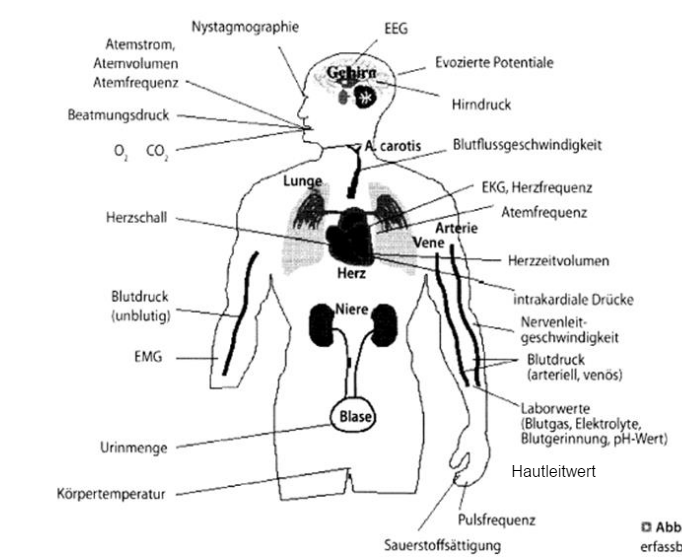
\includegraphics[scale=0.65]{Grafiken/beispielbiosig.png}

\subsection{Eigenschaften, Beschreibung, Darstellung}
Eigenschaften
\begin{itemize}
	\item Strukturgrößen: Länge, Fläche, menge, Volumen, Elastizität
	\item Funktionsgrößen: Temperatur, Druck, elektrische Potenziale, akustische Geräusche
	\item Beschreibung: Frequenz, Amplitude, Form, Auftrittszeitpunkt
	\item Darstellung: Zeit/Frequenzbereich, 2D oder 3D
	\item Auftreten: Stochastisch, stationär, periodisch, diskret
\end{itemize}

\subsection{Einteilung nach physikalischen Eigenschaften}
\begin{itemize}
	\item Bioakustische Signale: Herzschall, Lungengeräusche, Sprache
	\item Biochemische Signale: Stoffzusammensetzung, Konzentration
	\item Bioelektrische und biomagnetische Signale: Elektrische Potenziale, Ionenströme
	\item Biomechanische Signale: Größe, Form, Bewegung, Beschleunigung
	\item Biooptische Signale: Farbe, Lumineszenz
	\item Biothermische Signale: Körpertemperatur
\end{itemize}



\subsection{Messkette}
\begin{itemize}
	\item Applikation von Reizen, Strahlen, Substanzen, Wellen
	\item Primäres Messsignal Messen mit Fühler
	\item Signalverarbeiten (Linearisieren, Artefakterkennung, Rauschen entfernen)
	\item Biostatistik, Signalanalyse, Bildverarbeitung
	\item Bewertung
\end{itemize}


\subsection{Primäres Messsignal}
\begin{itemize}
	\item Medizin: Messsignal durch äußere Substanzen/Strahlen
	\item Biosignale: Invasiv, keine Anwendung äußerer Reize
	\item Meistens Signale, die vorhanden sind
	\item Primäres Messsignal: direkt vom Körper abgegriffen
\end{itemize}

\subsection{Reize}
\begin{itemize}
	\item Reize -> Reaktionen
	\item Mechanische, Elektrische, Akustische, Optische Reize, radioaktiv markierte Substanzen, Ultraschall, Röntgen, physische/psychische Reize
	\item Unwichtig für Benutzerschnittstellen, wichtig fürs Training
\end{itemize}

\subsection{Biosensoren}
\begin{itemize}
	\item Biosensoren erfassen Biosignale
	\item Mit Wandler verbunden oder ist direkt Wandler
	\item Wandler wandelt primär in sekundäres Messsignal um
	\item Sekundär Signal meist elektrisch
	\item Fühler ist eine biologische Detektionskomponente
\end{itemize}

\subsection{Biologische Detektionskomponente}
\begin{itemize}
	\item Sensitiv, spezifisch mit der Substanz
	\item Es können entstehen Wärme, Elektronen,Protonen, Lich, Gase, etc.
	\item Komponente besteht aus Enzymen, Mikroorganismen, Organellen, Zellverbände, Antikörper
\end{itemize}

\subsection{Anforderungen an Biosensoren}
\begin{itemize}
	\item Rückwirkungsfrei
	\item Reproduzierbar
	\item Konstantes Übertragungsverhalten
	\item Hohe Bioverträglichkeit
	\item Geringe Belastung
	\item Einfache Anwendung (Reinigung etc.)
	\item Entwicklungsziele für nächste Generation: Zuverlässiger, weniger Artefakte, Miniaturisierung, bessere Inkorporation, höhere Komplexität, Kanalanzahl, Berührungslosigkeit
\end{itemize}

\subsection{Wandler}
\begin{itemize}
	\item Wandeln primäres in sekundäres Messsignal
	\item Meist elektrisches Sekundärsignal
	\item Chemoelektrische Wandler, elektrische und magnetische Wandler, Mechanoelektrische Wandler, photoelektrische Wandler, thermoelektrische Wandler1
\end{itemize}

\subsection{Elektrische Wandler}
\begin{itemize}
	\item Ionenstrom->Elektronenstrom
	\item Ausdehnung (Dichte der Elektrodenplatzierung), Umgebungseinflüsse (Dreck, Tragekomfort) wichtig
	\item Größe: Mikro, Makroelektroden
	\item Platzierung: Oberflächen, Nadelelektroden
	\item Baufrom: Nadel, Schlaufe, Napf
	\item Materialien: Metallelektroden
\end{itemize}

\subsection{Mechanoelektrische Wandler}
\begin{itemize}
	\item Messung von Längenänderungen, Dehnungen, Druckschwankungen, Vibrationen, Blutfluss
	\item Besitzt Membran, die Kraftänderung detektiert (Auslenkung)
	\item Resistive Wandler: Membran = Spule, Längenveränderung des Dehnmessstreifens => Änderung des Widerstands
	\item Induktive Wandler: Membran = Spule, Verschiebung von Eisen/Ferritkern
	\item Kapazitive Wandler: Membran = Kondensator, Veränderung des Plattenabstandes => Kapazitätsänderung
	\item Kapazitive Wandler Beispiel: Kondensatormikrofon: Membran => Kondensator => Vibrationen verändern Entfernung der Platten => Kapazitätsänderung => Umwandlung in Spannungsschwankungen
	\item Piezoelektrische Wandler: Piezoelektrische Kristalle, mechanische Einflüsse in Richtung der polaren elektrischen Achsen bewirken Verformung => Verschiebung der Atome => Elektrische Ladung => Oberflächenladung
	\item Ladung ist Piezoelektrische Konstante $\times$ äußere Kraft
	\item Hall-Sonden: Nutzt Hall-Effekt: Strom durchflossen -> in orthogonales Magnetfeld => Spannung
	\item Photoelektrische Wandler: Erfassen Lichtabsorption und Lichtreflexion: Photowiderstand, Photodiode, Photoelement, Phototransistor: Lichtstärke => Stromänderung
	\item Thermoelektrische Wandler: Messung Atemstrom, Körpertemperatur
	\item Thermoelement: Temperaturdifferenz => Thermospannung
\end{itemize}

\subsection{Weitere Wandler - Indirekte Messung}
\begin{itemize}
	\item Biosignale oft indirekt erfasst
	\item Durch Einfluss von Strahlen, Wellen, radioaktive Stoffe
	\item PET, SPECT, MRT, CT; Angiographie
\end{itemize}

\subsection{Vorverarbeitung}
Elektrisches Sekundärsignal digitalisieren \\

\subsection{Vorverarbeitung - Differenzverstärker}
\begin{itemize}
	\item Zwei Eingänge, ein Ausgang
	\item $U_a = V*(U_e1-U_e2)$
	\item V Verstärkungsfaktor
	\item Wenn beide Eingänge gleich sind, Ausgangsspannung 0
	\item Brummen von Wechselstrom wird unterdrückt
	\item Linearität zwischen Eingangs und Ausgangssignal
	\item Verstärkung und Frequenzgang in Abhängigkeit des Biosignals
\end{itemize}

\subsection{Vorverarbeitung - Filterung}
\begin{itemize}
	\item Wirkt auf Frequenzkomponenten eines Signals
	\item Tiefpass- und Hochpassfilter
	\item Tiefpassfilter lässt tiefe Frequenzen passieren, dämpft hohe Frequenzen (EMG, EEG)
	\item Hochpassfilter lässt hohe Frequenzen passieren, dämpft langsame Wellen
\end{itemize}

Ideal: Linear, d.h. Änderung der Messgröße entspricht Änderung des Messwerts\\
Real nicht linear, da Außeneinwirkungen (Beispiel Messung Blutdruck, Gebilde zum Messen ist schwingungsfähig, daher leichte Änderungen)\\
Wesentliches Ziel ist Verbesserung der nicht-linearen Teile der Messkette

\subsection{Digitalisierung}
\begin{itemize}
	\item Sekundäres Messsignal ist kontinuierlich in Zeit und Amplitude
	\item Muss diskret im Computer sein
	\item Sampling und Quantisierung
	\item Quantisierung = Diskretisierung der y-Achse
	\item Sampling = Diskretisierung der x-Achse
\end{itemize}

\subsection{Digitale Signalverarbeitung}
\begin{itemize}
	\item Digitale Filterung
	\item Fensterung: Signal wird in Fenster unterteilt, um Zeitverlauf nachweisen zu können (Sprache, 16000 Samples/Sekunde -> 100 Fenster/Sekunde)
	\item Merkmalsextraktion (Wichtige Merkmale bezogen auf Kontext extrahieren)
	\item Kompression (Verringerung der Dimensionalität)
\end{itemize}

\subsection{Speicherung, Registrierung}
\begin{itemize}
	\item Direktschreibeverfahren: Ausgabe auf Registrierpapier
	\item Indirektschreibeverfahren: Photoschreiber und UV-Licht Schreiber
	\item Monitor: Analog oder Digitale Anzeige
	\item Speicherung auf Speichermedien
	\item Für Benutzerschnittstellen nur digitale Direktschreibung sinnvoll
\end{itemize}

\subsection{Übertragung}
\begin{itemize}
	\item Signale aus Körper
	\item Signale, die Auskunft geben über Person/implantierte Geräte
	\item Wired-Wireless, Bluetooth etc.
\end{itemize}

\subsection{Datenanalyse}
\begin{itemize}
	\item Messwerte: Zeitbereich/Frequenzbereich/Bildverarbeitung
	\item Beschreiben mit Systemen/Modellen/Simulationen
	\item Studien: Blindstudie (kein Placebo-Effekt), Doppelblindstudie (Untersucher kennt Faktoren nicht), Abhängige und unabhängige Stichproben, Langzeituntersuchungen
	\item Datenanalyse maschinell!
	\item Ablauf: Training + Klassifikation
\end{itemize}

\section{Erfassen von Biosignalen}


\subsection{Spracherkennung}
\begin{itemize}
	\item Traditionell: Mikrofon, Signal wird in elektrische Energie transformiert
	\item Probleme: Hörbarkeit (leise), Interferenz (Hintergrund), Privacy (öffentliche Orte)
	\item Alternativen?
\end{itemize}


\subsection{Stethoskop/NAM}
\begin{itemize}
	\item Kondensatormikrofon in Stethoskop
	\item "Hört" Körpervibrationen
	
\end{itemize}

\subsection{Bone-Conduction}
\begin{itemize}
	\item Resonanzkörper menschlicher Körper
\end{itemize}


\subsection{Geflüsterte Sprache}
\begin{itemize}
	\item keine/kleine Vibration der Stimmbänder
	\item gewisse Adaptionsschritte
	\item Throat microphone
	\item Close Talking microfone
\end{itemize}

\subsection{Bioelektrische Signale}
\begin{itemize}
	\item Potentialdifferenzen aus Nerven/Muskelvorgängen
	\item Elektroden leiten Signal ab
	\item Spannungsdifferenz benötigt
	\item Bipolare Ableitung: Potentialdifferenz zwischen zwei Elektroden auf elektrisch aktiven Gebieten
	\item Unipolare Ableitung/Referenzableitung: Eine Elektrode auf inaktivem Gebiet (Referenz)
\end{itemize}

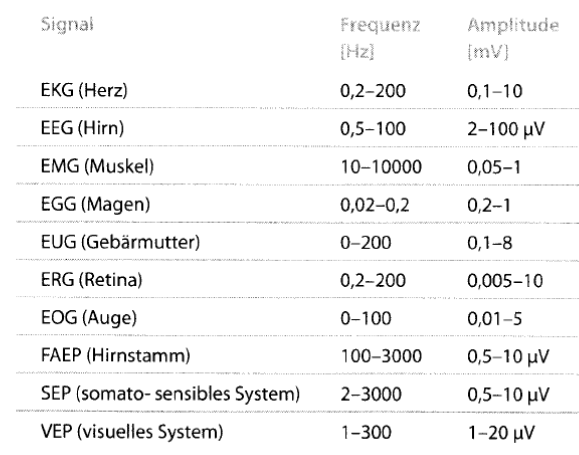
\includegraphics[scale=0.65]{Grafiken/bioelektrischesignalefreq.png}

\subsection{Erfassen elektrischer Felder}
\begin{itemize}
	\item Problem 1: Lokalisierung des elektrischen Feldes
	\item Anzahl Elektroden begrenzt
	\item Man geht bei EEG phänomenologisch vor, man erkennt Muster wieder, ohne alles zu verstehen
	\item Problem 2: Wandlung von Ionenstrom in Elektronenstrom
	\item Im Körper: elektr. Signalübertraung durch Ionenbewegungen
	\item Nötig, Ionen in Elektronenstrom zu wandeln, um erfassen zu können
	\item Elektroden erledigen dies
	\item Zwei Elektrodenarten:
	\item Redoxelektrode: Elektronen treten als Ladungsträger durch die Phasengrenze auf
	\item Ionen-Elektrode Ionen treten als Ladungsträger durch die Phasengrenze auf
\end{itemize}


\subsection{Nadelelektroden}
\begin{itemize}
	\item 2-6cm lang <1cm dick
	\item Verschiedene Seelen, Bipolare haben 2 Seelen
	\item Nadelelektronen unwichtig, da unkomfortabel (Einstich)
\end{itemize}


\subsection{Trockene/Feuchte Oberflächenelektroden}
\begin{itemize}
	\item Trockene: Direkter Körperkontakt, höherer Elektrode-haut Widerstand => Vorverstärker, groß, unhandlich
	\item Feuchte: Gel, meist verwendet
\end{itemize}

\subsection{Ionenelektrode}
\begin{itemize}
	\item Potenziale an Körperoberfläche gemessen
	\item Ankopplung mit Elektrolytpaste
	\item Metallischer Körper in Flüssigkeit => An Phasengrenze verschieben sich Ionen gegenseitig, Konzentrationen von Flüssigkeit/Metall ändern sich
	\item Ladungsverteilung
	\item Materialien haben chemische Potentiale
	\item => Ionenaustausch
	\item Gleichgewicht => Potentialdifferenz = Spannung (Galvani-Spannung)
	\item Stört Messung
	\item Messung über Referenzelektrode, da Bestimmung der Galvani-Spannung nicht möglich (Messung über Differenzen von zwei Galvani-Spannungen, zwischen bezugselektrode und untersuchende Elektrode)
	\item Durch Abnahme (Messen) von Strom, entsteht Stromfluss an Phasengrenze
	\item Dadurch Polarisation, Abweichung der Galvani Spannung
\end{itemize}

\subsection{Polarisation}
\begin{itemize}
	\item Thermodynamisches Gleichgewicht, kein Strom zuwischen Kathode und Anode
	\item Fließt durch Elektrode Strom, nicht Elektrodenpotenzial einen anderen Wert an
	\item Positiver(Anodischer) Strom = positive Abweichung
	\item Negativer (Kathodischer) Strom = Negative Abweichung
	\item Auslenkung der Elektrode heißt Polarisation oder Überspannung
	\item Durchtrittsüberspannung: Durchtritt durch Phasengrenze
	\item Diffusionsüberspannung: Ionentransport zur Phasengrenze
	\item Chemische Überspannung: Hemmung chemischer Reaktionen (Kristallisation)
	\item Polarisierbare Elektroden: Höher Überganswiderstand zwischen Körper und Elektrode, Verhalten wie Kondensator
	\item Bei Potenzialänderung erfolgt Stromfluss => Aufladung der Elektrode
	\item Unpolarisierbare Elektroden: Keine Hemmung des Ladungstransportes
	\item Ionenaustausch über Phasengrenze, Stromdichte S des Ladungstransports nur diffusionsbegrenz
	\item Reale Elektroden dazwischen (polarisierbar und unpolar.)
	\item Polarisierbare Metallelektrode: Positiv geladenene Metallionen in Elektrolytlösung: Osmostischer Druck und Feldkraft dagegen => elektrische Aufladung
	\item Aufbau einer entgegengesetzter Ladungsschickt im molekularen Abstand von der Phasengrenze
	\item Helmholtzsche Doppelschicht wie Kondensator => Polarisierbar
	\item Anwendungsbeispiel Ableitung höherfrequenter Signale
	\item Unpolarisierbare Metallelektrode: Metallelektrode wird mit Salz überzogen, Anion muss Bestandteil des Salzes sein
	\item Galvanispannungen kleiner und stabiler
	\item Geringere Überganswiderstände überall
	\item Ag/AgCl Elektroden für fast alle Signale einsetzbar
	\item Bei EEG wird Elektrolyt oder mit Kochsalzgetränktem Überzug verwendet
\end{itemize}

\subsection{Die Haut}
\begin{itemize}
	\item Wasserundurchlässig
	\item Leitfähigkeit durch Drüsen
	\item Kapazität umfasst Schichtaufbau der Haut
	\item Absenkung der Impedanz: Entfettung, Elektrodenpaste, Abtragen mit Sandpapier 
\end{itemize}

\subsection{Biokinetische Signale}
\begin{itemize}
	\item Messung von Bewegungen
	\item Direkte Erfassung EMG/EOG (Elektromyografie, Elektrookulografie)
	\item Indirekte Erfassung: Marker/Videoaufzeichnung
\end{itemize}


\subsection{Artefakte}
\begin{itemize}
	\item Störungen
	\item Ursachen Methoden, Proband, Speichertechnik (Kompression)
	\item Biologische Artefakte (vom Patienten)
	\item Technische Artefakte (Durch Geräte oder von außen)
	\item Biologische Artefakte (Augenbewegungen, Verspannungen, EKG Einstreuungen, Pulswellen, Schwitzen, Bewegungen)
	\item Technische Artefakte (Kontaktstellen, Kabeldefekte, Kabelbewegungen, fehlende Erdung, elektrostatische, magnetische oder elektromagnetische Wechselfelder
	\item Elektrische MEssmethode erzeugt viele dieser ARtefakte
\end{itemize}

\subsection{Artefaktbereinigung}
\begin{itemize}
	\item Testmethoedn anpassen (Abschirmen, möglichst viel konstant halten (Tageszeit, helligkeit)
	\item Technische Möglichkeiten: Bandsperrfilter, Hintergrundaktivitäten selektieren, Adaptive Filter, spezielle Algorithmen
	\item Manuelle/Automatische Artefaktrejektion
\end{itemize}

\section{Nervensystem, Informationsfluss im menschlichen Körper}

\subsection{Bausteine}
\begin{itemize}
	\item Neuronen: Transport und Verarbeitung von Signalen/Informationen
	\item Gliazellen: Hilfsapparat für Neuronen, Schutz, Versorgung, Stütze
\end{itemize}


\subsection{Neuronen}
\begin{itemize}
	\item Zellkörper(Soma): Verdickung, Verarbeitung von Informationen, wesentliche Stoffwechselvorgänge, enthält Zellkern
	\item Axon (Sender): Langer Zellfortsatz, transferiert Informationen vom Zellkörper zu anderen Zellen
	\item Dendriten (Empfänger): Zellfortsätze aus dem Zellkörper, sammeln Informationen von anderen Neuronen, stark bedornt, andere Neuronen können andocken
	\item Myelinscheide: umhüllt Axon, dient Beschleunigung der Leitungsgeschwindigkeit des Axons
	\item Vier Prinzipien der neuronalen Organisation:
	Grundlegende Strukturelle/funktionelle Einheit des Gehirns \\
	Axonenendigungen kommunizieren mit Dendriten anderer Neuronen nur an bestimmten Stellen, den Synapsen \\
	Verbindungsspezifität: Jede Nervenzelle kommuniziert nur mit ganz bestimmten anderen (spezielle Schaltkreise) \\
	Signalübertragung nur in eine Richtung
\end{itemize}

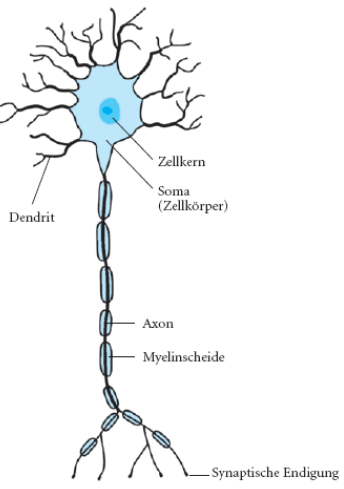
\includegraphics[scale=0.65]{Grafiken/neuron.png}


\subsection{Klassifikation}
\begin{itemize}
	\item Nach äußerer Gestalt (Pyramiden, Stern, ...)
	\item Nach Verbindungen:
	\item Sensorische Neurone: Informationsweitergabe über physikalische oder chemische Reize
	\item Motoneurone: Gehirn und Rückenmark, Steuern Aktivität von Muskel und Drüsenzellen
	\item Interneurone: Dienen als Umschaltstation zwischen sensorischen und motorischen
\end{itemize}


\subsection{Gliazellen}
\begin{itemize}
	\item "Führungselemente" beim Wachstum von Neuronen
	\item Stützelemente des Nervensystems
	\item Transportmedium 
	\item bilden Myelinscheiden
	\item Beeinflussung der Effektivität synaptischer Kontakte
	\item Wirken bei Blut/Hirn Schranke mit, schirmen Nervensystem von schädl. Stoffen im Blut ab
\end{itemize}

\subsection{Weiße/Graue Substanz}
\begin{itemize}
	\item Graue Substanz: Großhirnrinde (Cortex) und Kerne, besteht aus Neuronen Zellkörpern
	\item Weiße Substanz: Unterhalb des Cortex, bettet graue Substanz ein, besteht aus Nervenfasern
\end{itemize}


\subsection{Ruhepotential}
\begin{itemize}
	\item Ionenkonzentration im Zellinneren ungleich Zelläußeren => Potentialdifferenz
	\item = Membranpotential (Mensch -70mV Ruhepotential) (Zellinnere negativ außen)
	\item Zelle elektrisch polarisiert
	
\end{itemize}



\subsection{Messung}
\begin{itemize}
	\item Einstich in Zellinnere, zweite Elektrode außerhalb
\end{itemize}


\subsection{Permeabilitätsunterschiede}
\begin{itemize}
	\item Keine Ladungsausgleich da: Zellmembran nicht gleichermaßen durchlässig
	\item Ruhepotential aus unterschiedlcihen Verteilungen von Na, K, Cl, Proteinen
	\item Hoch permeabel: K+, Cl-
	\item Niedrig permeabel: Na+
	\item Undurchlässig: Proteinanionen
	\item Zellinnere K+, negative geladene Proteine
	\item Zelläußere: Na+, Cl-, Ca2+
	\item Elektrostatische Kräfte
	\item Thermische Bewegung-> Körperwärme
\end{itemize}

\subsection{Natrium-Kalium-Pumpe}
\begin{itemize}
	\item K+ in negativen zellinneren
	\item Cl- im positiven Äußeren
	\item Na+ außen (trotz Ladung)
	\item Natrium-Kalium-Pumpe befördert Na+ aus der Zelle ins Äußere (aktiver Transport)
	\item Membranproteine zwischen innen und außenseite (besitzen 3 Bindestellen für Na+ innen, 2 Bindungsstellen für K+ außen)
	\item K+ wandert durch Kaliumkanäle aus Zellinneren (passiver transport)
\end{itemize}

\subsection{Passiver Signaltransport}
\begin{itemize}
	\item Kein Energieverbrauch
	\item Potentialänderung
	\item Leitung schnell und verlustreich
	\item Nur bei kurzen Distanzen möglich (<1mm, z.B. Membranen der Dendriten)
	\item z.B. im Gehirn (informationsverarbeitung auf engem Raum)
\end{itemize}

\subsection{Aktionspotential (Spike)}
\begin{itemize}
	\item Zellen erzeugen Potenzialspitzen
	\item Verlustarme Weiterleitung
	\item Über lange Distanzen möglich
	
	\item Erregbare Nervenzellen reagieren uaf Reiz (Ionenleitfähigkeit der Membran ändert sich)
	\item Können weitaus höhere Spannung als der ursprüngliche Reiz verursachen
	\item Spannungsänderung durch Reiz => von Innen nach außen gerichteter Strom durch Membran
	\item 3 Phasen
	\item Depolarisation: schnell: Ionentör öffnet sich, Natriumeinstrom: Potential wird größer
	\item Repolarisation: langsam: Kaliumtore öffnen sich, Kaliumausström: Potential fällt ab
	\item Nachhyperpolarisation: Kaliumtore schließen sich nur langsam: Potential fällt unter Ruhepotential
	\item Nach Aktionspotential: Membran schwer/überhaupt nicht erregbar, Refraktärphase
	
\end{itemize}

\subsection{Saltatorische Erregungsleitung}
\begin{itemize}
	\item Ausbreitung des Aktionspotential entlang des Axons ist sprunghaft
	\item Myelinscheiden wie Isolatoren
	\item An Ranvier-Schnürringen sind unmyelinisierte Stellen (Hohe Konzentration an sspannunggesteuerten Na-Kanälen, Aktionspotential wird wieder aufgefrischt)
	
\end{itemize}

\subsection{Aktionspotentiale Eigenschaften}
\begin{itemize}
	\item Alles- oder Nichts: Stärke des Reizes keien Auswirkung auf Höhe AP
	\item Stärke des Reizes bestimmt Geschwindigkeit des AP, (Länge Refraktärzeit)
	\item Reizstärke in Frequenz der AP umkodiert
\end{itemize}

\subsection{Informationsübertragung: Synapse}
\begin{itemize}
	\item Signalübertragung durch Synapsen
	\item Definition Synapse: Verbindungsstelle zwischen zwei Neuronen oder einem Neuron und einer Zelle des Erfolgsorgans (z.B. Muskelzelle) an der Information weitergegeben wird
	\item Axon - Dendrit oder Axon - Soma
	\item Elektrische Synapse
	\item Chemische Synapse
\end{itemize}

\subsection{Elektrische Synapse}
\begin{itemize}
	\item Nahe Zellmembranen
	\item Röhrenartige Verbindung
	\item Schnell
	\item Informationsübertragung in beide Richtungen
	\item Synchronisation von Zellverbänden mit identischen Funktionen: Muskelzellen des Herzens, Muskelzellen der inneren Organe, Neuronenverbände im Gehirn
\end{itemize}

\subsection{Chemische Synapsen}
\begin{itemize}
	\item Spalt größer als bei elektrische Synapse
	\item Spalt wird mit chemischen Botenstoffen überbrückt
	\item Ausganszelle sendet Botenstoff, löst Prozess an Membran von Empfängerzelle aus -> Ionenwanderung
	\item Asymmetrisch
	\item Nicht so schnell
	\item Zentralnervensystem Informationsverarbeitung
	\item Präsynaptische Endigung (Sender)
	\item Postsynaptischer Membranbereich (Empfänger)
	\item Ablauf Informationsübertragung:
	\item Membranerregung in präsynaptische Endigung
	\item Neurotransmitter in synaptischen Spalt
	\item Verteilt sich darin
	\item Erreich Empfängermoleküle (Rezeptoren) an postsynaptischer Membran
	\item Transmitterstoffe wirken an Repezeptoren
	\item Ionenkanäle öffnen sich -> Potentialveränderung -> evtl. neues AP
	\item Chemische Übertragung: schnell, gezielt, kurz
	\item Neurotransmitter ist in den Vesikeln der präsynaptischen Endigung gespeichert
\end{itemize}




%__________________________________BENNE



\section{11 - HMM (Hidden Markov Models)}
	\begin{itemize}
		\item Modellieren Sequenz von Datenpunkten
		\item benötigen zugrundeliegendes state modeling
		\item oft zusammen mit GMMs verwendet
	\end{itemize}
	
\subsection{Sequenzmodellierung und State-Modelierung}
	\begin{itemize}
		\item Sequenzmodellierung ist in typischer Signalverarbeitungskette letzte Schritt nach Datenverarbeitung und State Modeling 
		\item Klassifikation und Sequenzmodellierung eng miteinander verbunden
	\end{itemize}

\subsection{Dynamic Time Warping}
	\begin{itemize}
		\item einfaches Verfahren zum Vergleich von Sequenzen
		\item Algorithmen in der HMM-Modellierung sehr ähnlich zu DTW
		\item Wir haben: Aufnahmen von Sprachsignalen - Trainingsdaten (Beispielaufnahmen mit bekanntem Inhalt) + Testdaten (Aufnahmen mit unbekanntem Inhalt)
		\item Ziel: Wir wollen die Distanz einer unbekannten Sequenz und einer Beispielsequenz berechnen
		\item Frame für Frame-Vergleich Probleme: Signale sind unterschiedlich lang + Anfang und Ende der Äußerung nicht bekannt
		\item Faggot-Lösung: Lineares Alignment - für fast alle Zwecke aber viel zu unflexibel
		\item Killer-Lösung: DTW
				\begin{itemize}	
					\item basiert auf Prinzip des dynamischen Programmierens (DP) bzw. der minimalen Editierdistanz
					\item Pfade durch eine Matrix von möglichen Zuordnungen berechnet
					\item Ergebnis: Distanzmaß zwischen den beiden Äußerungen
				\end{itemize}
	
		\item Ziel: Finde Distanz zwischen den beiden Äußerungen (je niedriger desto besser)
		\item Problem: Alle Pfade müssen betrachtet werden um den Besten zu finden
		\item Lösung:
				\begin{itemize}
					\item Berechne für jede Zeit $t$ die kumulativen Distanzen $\alpha(s,t)$, die die Distanz der Teiläußerungen bis zu den Zuständen q(s,t) (s=,1,..,S)  beschreiben
					\item Die Distanzen für Zeitpunkt t+1 berechnen sich iterativ aus denen für Zeitpunkt t und hier wird Minimierung der Distanz durchgeführt
				\end{itemize}
					\item Benötige Distanzmaß $d(s,t)$ für den beobachteten Frame t und den Referenzframe s (z.B. euklidische Distanz)
 		\end{itemize}
 		\centering
 		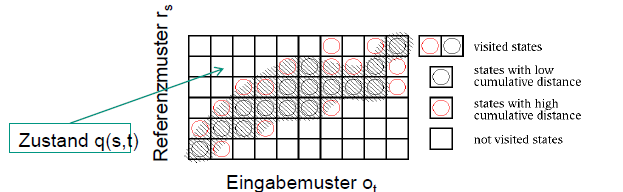
\includegraphics[scale=0.65]{Grafiken/DTW_Beispiel.png}
 		
 		\begin{itemize}
 			\item Welche Übergänge zwischen Frames sind möglich? Was haben sie für Distanz-Kosten?
 			\item Erlaubt sind überlicherweise:
 				\begin{itemize}
 					\item Ersetzung: Kosten = d(.,.) (praktisch immer > 0)
 					\item Einfügung/Auslassung eines Frames: Kosten können in der Praxis ignoriert werden
 					\item Einfügung/Auslassung mehrerer Frames: evtl. Extra-penalty, max. Zahl von Frames, die ausgelassen werden dürfen
 				\end{itemize}
 		\end{itemize}
\vspace{5px}
\flushleft Ablauf des Algorithmus:
 			\begin{itemize}
 				\item Initialisierung: Beginne bei Startzustand $q(0,0)$, $t:=0$, $\alpha(0,0):=d(0,0), \alpha(x,0)=\infty$
 				\item Für jeden Zustand $q(s,t)$:
 					\begin{itemize}
 						\item Betrachte jeden erlaubten Zustandsübergang $q(s',t-1) -> q(s,t)$
 						\item Finde min. Distanz zu $q(s,t)$
 						\item Bis Teildistanz $\alpha(s,t)$ einen gewissen Grenzwert überschreitet
 					\end{itemize}
 				\item weitere Einschränkungen des Suchraums denkbar
 				\item Komponenten der Zustandsmatrix Schritt für Schritt berechenbar (zeiteffizient + speichereffizient)
 			\end{itemize}
 		\begin{itemize}
 			\item Anwendung in der Spracherkennung
 			\item z.B. heute noch praktisch bei der Erkennung von sehr kleinen Vokabularen
		\end{itemize} 	
		
\vspace{5px}
\flushleft Probleme bei Unterscheidung einer kleinen Menge von Wörtern:
		\begin{itemize}
			\item benötigt eine Endpunktdetektion
			\item wird sehr ineffizient wenn viele Trainingsbeispiele vorhanden sind - großes Vok. braucht extrem viele Trainingsbeispiele
			\item Trainingsdaten können nicht zwischen verschiedenen Referenzen geteilt werden
			\item Erkennung unbekannter Wörter ist nicht möglich
			\item ungeeignet für kontinuierliche Sprache
			\item sehr kurze Wörter sind schwer zu trainieren
		\end{itemize}
	$\Rightarrow$ Andere Methode wird benötigt die es ermöglicht, kleinere Einheiten (Silben, Phoneme) zu trainieren und zu erkennen 		

\subsection{Markov-Modelle}
Sprachproduktion als stochastischer Prozess
	\begin{itemize}
		\item Beobachtungen zur Sprachproduktion:
		\begin{itemize}
			\item das gleiche Wort/Phonem hört sich jedesmal anders an
			\item in einem gegebenen Zustand können verschiedene Laute mit 		unterschiedlicher Wahrscheinlichkeit beobachtet werden
			\item der Produktionsprozess kann Übergänge aus einem Zustand in einen anderen machen, aber nicht alle denkbaren Übergänge sind möglich, zumindest nicht gleich wahrscheinlich
		\end{itemize}
		\item Sprachprozess befindet sich zu jedem Zeitpunkt in einem Zustand
		\item In jedem Zustand werden Laute ausgegeben entsprechend einer gewissen Wahrscheinlichkeit: Emissionswahrscheinlichkeit
		\item Die Übergänge zwischen Zuständen erfolgen auch entsprechend einer gewissen Wahrscheinlichkeitsverteilung: Übergangs- oder Transitionswahrscheinlichkeiten
		\item Markov-Modelle:
			\begin{itemize}
				\item Es gibt eine diskrete Zustandsmenge ${s_1, ... ,s_N}$
				\item Wir beobachten eine probabilistische Zustandssequenz $O = (o_1,...,o_T), o_i \in  {1,...,N}$
				\item Markov-Annahme: Wahrscheinlich, dass wir zum Zeitpunkt t in einem gewissen Zustand sind, hängt nur von vorhergehendem Zustand ab
				\item Verteilung soll stationär (zeitunabhängig) sein
			\end{itemize}
	\end{itemize}
	
\subsection{Hidden-Markov-Modelle}
Markov-Modelle und Spracherkennung
	\begin{itemize}
		\item Zustand $<=>$ Beobachtung
		\item In der Sprache haben wir aber ein Kontinuum an möglichen Tokens (typischerweise Sprachsignalframes), die endlich vielen Zuständen (Phonemen) zugeordnet werden sollen
		\item In der Sprache sind die Zustände versteckt (hidden)
	\end{itemize}
	
Hidden-Markov-Modelle (HMM) 
	\begin{itemize}
		\item sind ein doppelter stochastischer Prozess
			\begin{itemize}
				\item Zustandsabfolge probabilistisch
				\item Jeder Zustand emittiert seine Beobachtung: Diese Emission ist ebenfalls probabilistisch
				\item Zustandsfolge ist versteck (hidden)
			\end{itemize}
		\item Sind Markov-Modelle (1. Ordnung)
			\begin{itemize}
				\item Wahrscheinlichkeiten für den Eintritt in den nächsten Zustand hängen nur vom aktuellen Zustand ab
			\end{itemize}
		\item Nichtbeobachtbarkeit der Zustandsfolge hat eine Reihe von Konsequenzen		
			\begin{itemize}
				\item Sprachdekodierung mit HMMs: Anhand der Beobachtungen auf eine mögliche Zustandssequenz rückschließen (dabei wird man nie die exakte Lösung erhalten, sondern nur eine mit höchster Wahrscheinlichkeit)
				\item Training von HMMs: Kennen zwar die durchlaufene Zustandsfolge, aber nicht die Zeitpunkte der Zustandsübergänge
			\end{itemize}
			\centering 
			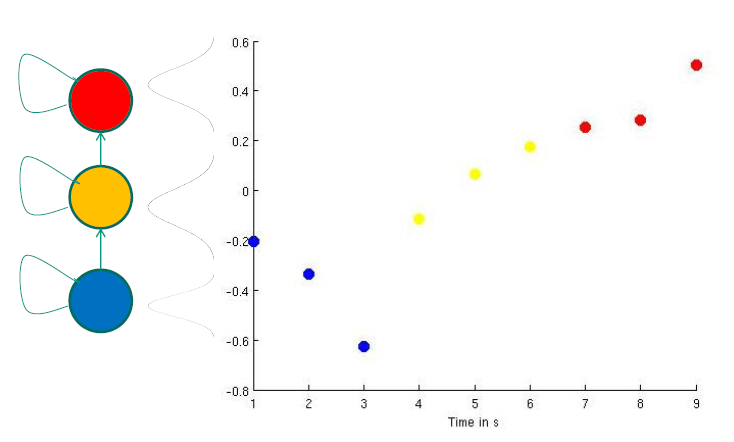
\includegraphics[scale=0.5]{Grafiken/hmm-darstellung.png}
	\end{itemize}

Formale Definition:
	\begin{itemize}
		\item HMM $\lambda = (S,\pi, A,B,V)$
		\item $S={s_1,...,s_N}$ - Menge aller möglichen Zustände
		\item $\pi$: $\pi(s_i) = P(q_1 = s_i)$ - Anfangsverteilung bei t=1
		\item $A=((a_{ij})), 1 \leq i, j \leq n$ - Matrix von Übergangswahrscheinlichkeiten
		\item $B=(b_i)$ - Vektor von Ausgabewahrscheinlichkeiten, d.h. $b_i(v)=P(o_t = v | q_t = s_i)$. Dabei ist $v \in V$
		\item V - Vokabular, Menge der Ausgabesymbole (diskret oder kontinuierlich)
	\end{itemize}

Diskrete HMMs:$V = {x_1,x_2, ...,x_v}$, dann sind die $b_i$ diskrete Wahrscheinlichkeiten


Kontinuierliche HMMs: $V=R^d$, dann sind die $b_i$ stetige Wahrscheinlichkeitsdichten

\begin{itemize}
	\item Für die Anfangswahrscheinlichkeiten gilt $\sum_i \pi(s_i) = 1$. Vereinfachend nimmt man oft einfach: $\pi(s_1) = 1 \enspace , \enspace \pi(s_j) = 0 \enspace , \enspace j \neq 0$, d.h. es gibt einen ausgezeichneten Startzustand)
	\item Es gilt $\sum_j a_{ij} = 1$ für alle i und meistens ist $a_{ij} = 0$ für die meisten Folgezustände j
\end{itemize}
Die Struktur eines HMMs nennt man Topologie:
	\begin{itemize}
		\item Lineares Modell:  \\ 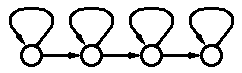
\includegraphics[scale=0.3]{Grafiken/hmm-struktur.png} 
		\item Links-nach-Rechts-Modell: \\ 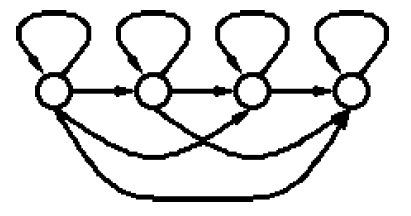
\includegraphics[scale=0.2]{Grafiken/hmm-lnr.png} 
		\item Alternative Pfade: \\ 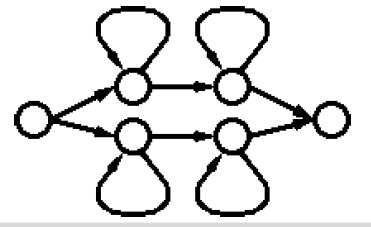
\includegraphics[scale=0.2]{Grafiken/hmm-ap.png}
		\item Bakis model (lin. Modell + kann je 1 Zustand übersprungen werden): \\ 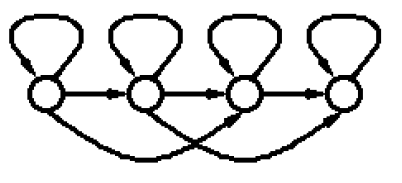
\includegraphics[scale=0.2]{Grafiken/hmm-bakis.png}   
		\item Ergodisches Modell (Jeder Zustand ist von jedem anderen Zustand erreichbar): \\
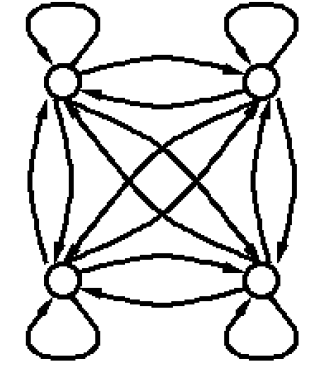
\includegraphics[scale=0.2]{Grafiken/hmm-em.png} 
	\end{itemize}

HMM-Theorie kennt drei Hauptaufgaben: Evaluationsproblem, Dekodierungsproblem, Optimierungsproblem

Evalutationsproblem: Berechne die Wahrscheinlichkeit der Beobachtung $P(O|\lambda)$
	\begin{itemize}
		\item Entspricht der Durchführung des DTW-Algorithmus
		\item Forward-Algorithmus löst dieses Problem
		\item Herausforderung: Wir müssen die Wahrscheinlichkeit der Beobachtung entlang aller möglichen Pfade berechnen
		\item Sehr aufwendig - Finden effizienter Algorithmen
		\item Frage: Wie summieren wir die Wahrscheinlichkeiten entlang aller möglichen Pfade effizient auf?
		\item Lösung: Ansatz ist wie beim dyn. Programmieren:
			\begin{itemize}
				\item Berechne iterativ für jeden Frame und jeden Zustand die Vorwärts-Teilwahrscheinlichkeiten (forward probabilities) $\alpha$
				\item Dann ergibt sich eine Matrix A der Vorwärtswahrscheinlichkeiten \\ 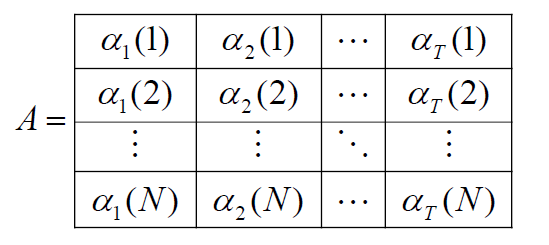
\includegraphics[scale=0.2]{Grafiken/hmm-fa-A.png}
				\item $\alpha_t(j)$ bezeichnet die Wahrscheinlichkeit, bei gegebener Teilbeobachtung zum Zeitpunkt t im Zustand j zu sein. Zur Berechnung iteriert man über die Zeit:
				\item Init: $\alpha_1(j) = b_j(o_1) \pi(s_j)$
				\item Induktion: $\alpha_t(j) = b_j(o_t) \cdot \sum_{i=1..n} a_{ij} \alpha_{t-1}(i)$ 
				\item Ergebnis: $p(o_1,o_2,...,o_T|\lambda) = \sum_{j=1..n} \alpha_T(j)$
				\item Komplexität: $O(N^2T)$
			\end{itemize}
	\end{itemize}

Dekodierungsproblem: Berechne die wahrscheinlichste Zustandsfolge bei der gegebenen Beobachtung $(q_1^*,...,q_{t-1}^*,q_t^*) = arg \max_{q_1,...,q_t} P(q_1,...,q_t|O,\lambda)$. Viterbi-Algorithmus:
	\begin{itemize}
		\item Definiere: $z_t(j) := \max_{q_1,...,q_{t-1}} P(q_1,...,q_{t-1}, q_t = j, o_1,...,o_t)$
		\item $z_t$ ist die maximale Wahrscheinlichkeit (maximiert über alle Zustandsfolgen bis Zeitpunkt t), mit der bei der gegebenen Teilbeobachtung zum Zeitpunkt t der Zustand j erreicht wird
		\item Man kann $z_t(j)$ iterativ berechnen, indem man alle möglichen Vorgängerzustände betrachtet und maximiert: \\
			$z_t(j) = \max_i z_{t-1}(i) \cdot a_{ij} \cdot b_j(o_t)$\\
			$z_1(j) = \pi(s_j) \cdot b_j(o_1)$
		\item Ergibt sich eine Matrix Z, ähnlich wie beim Forward-Algorithmus \\
		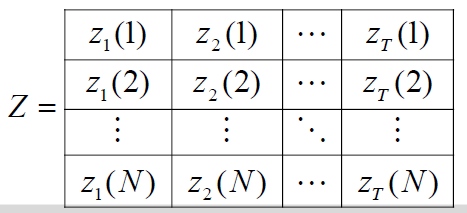
\includegraphics[scale=0.2]{Grafiken/viterbi-algo.png}
		\item Rechenaufwand: $O(N^2T)$
		\item Außerdem speichern wir für jeden Zustand den optimalen Vorgängerzustand: $r_t(j) = argmax_t (z_{t-1}(i) a_{ij})$
		\item Wenn alle $z_t$ und $r_t$ berechnet sind, kann Rückwärtszeiger $r_t$ benutzt werden, um die gesuchte optimale Zustandsfolge zu berechnen
		\item Beginne beim letzten Zeitpunkt T und suche den wahrscheinlichsten Zustand. Dann gehe entlang der Rückwärtszeiger schrittweise zurück: \\
		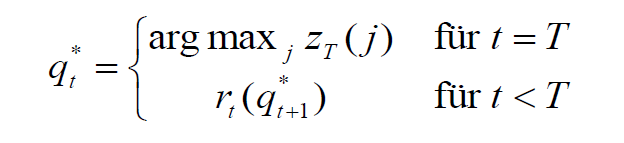
\includegraphics[scale=0.2]{Grafiken/viterbi-algo-qt.png}
	\end{itemize}

Optimierungsproblem: Finde ein HMM $\lambda^{'}$, so dass $P(O|\lambda^{'})> P(O|\lambda)$ (Ein gegebenens HMM $\lambda$ soll verbessert werden)
	\begin{itemize}
		\item Welche Parameter können trainiert werden: Übergangswahr., Emissionswahr., Anfangswahr.
		\item Probleme bei der Optimierung: unbekannt zu welchem Zeitpunkt wir in welchem Zustand sind, Wahrscheinlichkeit berechenbar dass zu Zeitpunkt t im Zustand $s_j$ (diese Information können wir zur Gewichtung nutzen)
		\item Lösung des Optimierungsproblem besteht aus 2 Schritten:
		\item Estimation Step: Berechne die Zuordnungswahrscheinlichkeit von Trainingsdaten zu HMM-Zuständen
			\begin{itemize}
				\item Trainingsbeobachtung $O=(o_1,...,o_T)$
				\item für jedes Sample die Wahrscheinlichkeit berechnen, dass es einem gewissen HMM-Zustand zuzuordnen ist
				\item für jede Kombination von aufeinanderfolgenden Samples die Wahrscheinlichkeit berechnen, dass sie einem gewissen Zustandsübergang zuzuordnen sind
			\end{itemize}
		\item Maximization Step: Optimiere die Parameter von Emissionswahrscheinlichkeiten, (Übergangswahrscheinlichkeiten und Anfangswahrscheinlichkeiten)
	\end{itemize}
 
Forward-Backward-Algorithmus:
	\begin{itemize}
		\item Berechnet die Zuordnungswahrscheinlichkeiten von Trainingsdaten zu HMM-Zuständen, löst also den Expectiation Step
		\item Betrachten wir eine Beobachtung $o=(o_1,...,o_T)$
		\item Gesucht sind 2 Parameter:
			\begin{itemize}
				\item $Y_t(j) = P (q_t=j|o_1,...,o_T,\lambda)$ ist die Wahrscheinlichkeit, dass der Beobachtungsvektor $o_t$ zum Zustand j gehört
				\item $\xi_t(i,j) = P (q_t=i,q_{t+1}=j | o_1,...,o_T,\lambda)$ ist die Wahrscheinlichkeit, dass zum Zeitpunkt t im Zustand i befinden und dann in den Zustand j übergehen
			\end{itemize}
		\item Beide Wahrscheinlichkeiten hängen von der gesamten Beobachtung o ab
		\item Berechnung von $y$ und $\xi$
			\begin{itemize}
				\item Forward-Algorithmus berechnet die Wahrscheinlichkeit, nach der Teilbeobachtung $(o_1,...,o_t)$ also zum Zeitpunkt t im Zustand j zu sein
				\item Backward-Algorithmus berechnet die Wahrscheinlichkeiten im Zustand j zu sein und dann die Teilbeobachtung $(o_{t+1},...,o_T)$ zu machen
				\item Kombination der beiden ergibt Forward-Backward-Algorithmus, der $Y_t(j)$ berechnet
				\item Berechne $P(q_t=j|o_1,...,o_T,\lambda)$ druch Aufspaltung in Forward-Teil (bis Zeit t) und Backward-Teil (nach Zeit t).
				\item $\alpha_t(j) := P(q_t=j,o_1,...,o_t|\lambda)$ \\
					  $\beta_t(j) := P(q_{t+1}=j,o_1,...,o_T|\lambda)$ \\
					  $\Rightarrow P(q_t=j|o_1,...,o_T,\lambda) = \alpha_t(j) \cdot  \beta_t(j)$. Anwendung der Bayes-Regel ergibt: \\ \vspace{3px}
				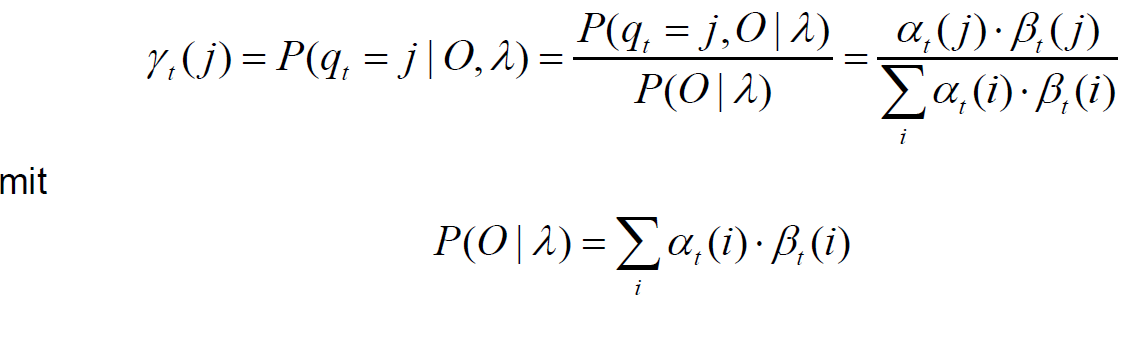
\includegraphics[scale=0.2]{Grafiken/forward-backward-algo.png}	  	
				\item $\beta_t$ können ähnlich wie die $\alpha_t$ rekursiv berechnet werden, aber rückwärts:
					\begin{itemize}
						\item Init: $\beta_T(i) = 1$ für alle Zustände i
						\item Induktion: $\beta_t(t) = \sum_{j=1..n} a_{ij} b_j (o_{t+1})\beta_{t+1}(j), \enspace t=T-1,..., 1$
						\item Durch Aufsummieren: $\Rightarrow p(o_{t+1},o_{t+2},...,o_T|\lambda) = \sum_{j=1..n} \beta_T(j)$
					\end{itemize}			
				\item[] 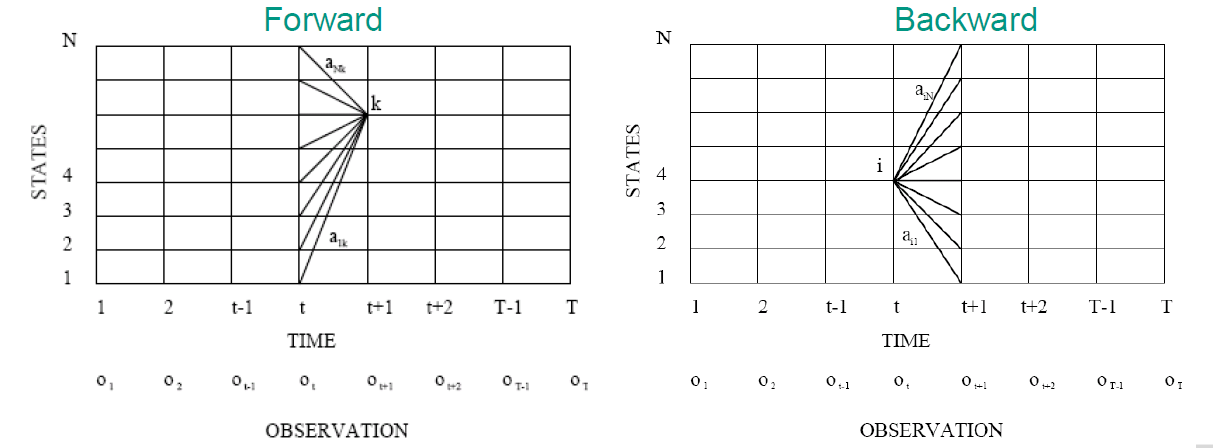
\includegraphics[scale=0.25]{Grafiken/forward-backward-beta.png}	  		 		\item $\xi_t(i,j)$: auch mit Forward-Backward-Algorithmus $\xi_t(i,j) = P(q_t = i,q_{t+1} = j|O,\lambda)$
				\item[] 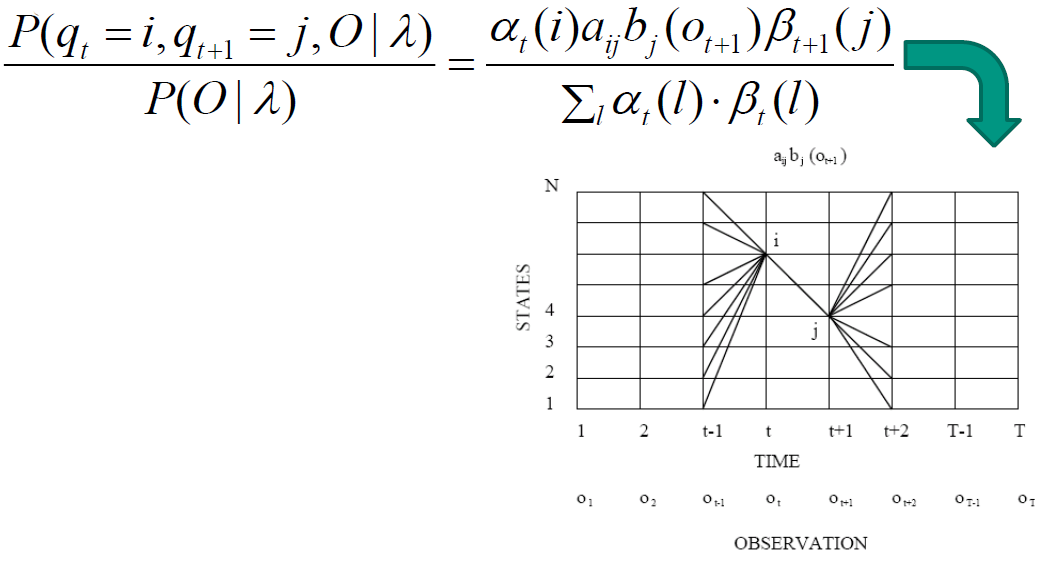
\includegraphics[scale=0.2]{Grafiken/xis.png}
			\end{itemize}
	\end{itemize}

\underline{Optimierung des HMMs:}
	\begin{itemize}
		\item Trainingsdaten den HMM-Zuständen und Zustandsübergängen zugeordnet
		\item Das war der Expectation Step des Algorithmus
		\item Führe nun Maximierung der HMM-Ausgabewahrscheinlichkeit durch (Maximization Step)
		\item Zuordnung der Samples zu HMM-Zuständen, gegeben durch $\alpha_t(j),\beta_t(j),Y_(j)$
		\item Falls Emissionswahrscheinlichkeiten durch Gauss-Mischverteilungen modellieren, dann verwende EM-Algorithmus zum Training
	\end{itemize}
	
\underline{Optimierung der Emissionswahrscheinlichkeiten:} \\
Betrachten Emissionswahrscheinlichkeiten $B^{'}=(b_1^{'},...,b_N^{'})$ bei diskretem Ausgabealphabet V. Zu jedem Zustand i = 1,...,N gehört eine Verteilung $b_i$, so dass $b_i(v_k) \in  [0,1]$ die Wahrscheinlichkeit angibt im Zustand i die Beobachtung $v_k$ zu machen. \\
Danach werden die $b_i^{'}$ bestimmt: 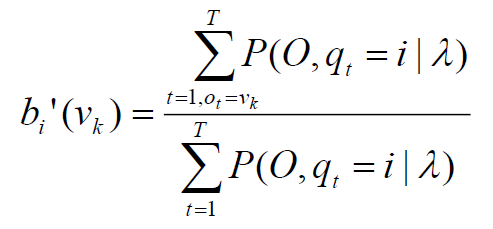
\includegraphics[scale=0.2]{Grafiken/bis.png}\\
Das heißt, $b_i^{'}(v_k)$ entspricht dem Anteil der Emissionen von $v_k$ an der Gesamtzahl der "Besuche" von Zustand i.
	
	
\underline{Optimierung der Übergangswahrscheinlichkeiten:} 	
	\begin{itemize}
		\item $sum_{t=1..T-1} \xi_t(i,j)$ ist der Erwartungswert der Anzahl der Transitionen von i nach j
		\item Der neue Wert $a_{ij}^{'}$ ist der Anteil der Transitionen von i nach j, normalisiert durch die Gesamtzahl der Transitionen (=Besuche) von i 
		\item Summiere über alle Zeitpunkte t=1,...,T: $a_{ij}^{'} = \frac{\sum_t \xi_t(i,j)}{\sum_t \gamma_t(i)}$
		\item Der neue Wert $\pi^{'}(i)$ ist dementsprechend die Anzahl der Besuche von i zur Zeit t = 1, also $\pi_t^{'} = \gamma_1(i) = \frac{\alpha_1(i)\beta_1(i)}{\sum_l \alpha_1(l)\beta_1(l)}$
	\end{itemize}
 		
\underline{Baum-Welch-Regeln:} \\ 	
	\begin{itemize}
		\item Alle Parameter des HMMs an die aktuelle probabilistische Zuordnung der Samples, gegeben durch $\gamma_t(i)$, angepasst. Es ergibt sich also ein neues HMM: $\lambda^{'} = (S,\pi^{'},A^{'},B^{'},V)$
		\item Dieser Algorithmus wird, wie es für EM-Algorithmen typisch ist, so lange iterativ wiederholt, bis ein Abbruchkriterium erfüllt ist
		\item Die Regeln der letzten "Folien" sind die Baum-Welch-Regeln
	\end{itemize}
	
\underline{Training von HMMs mit Viterbi:} \\ 
	\begin{itemize}
		\item Viterbi, der immer nur maximale Wahrscheinlichkeiten betrachtet, geht viel schneller als Forward-Backward-Algorithmus
		\item In der Spracherkennung ist Viterbi-Training Standard
	\end{itemize}
	
\section{12 - Spracherkennung}
\subsection{Schall als Luftdruckwelle} 

\underline{Was ist Schall?} \\ 
	\begin{itemize}
		\item Druckwelle, die von einem vibrierenden Objekt erzeugt wird
		\item Vibration überträgt sich auf Partikel des umgebenden Trägermediums (z.B. Luft) - Energietransport über Medium findet statt
		\item Partikel parallel zur Ausbreitungsrichtung der Welle - spricht man von Longitudinalwelle
		\item Longitudinalwelle besteht aus Kompressionen (Verdichtungen) + Rarefaktionen (Verdünnungen) der Luft
		\item Lässt sich durch Sinusfkt. beschreiben
		\item Amplitude entspricht der Dichte der Luft an der betreffenden Stelle
		\item Ausbreitungsgeschwindigkeit in der Luft: 331,5 + 0,6 T m/s, T = Temperatur in C
	\end{itemize}

\underline{Messung der Schallintensität} \\  
 	\begin{itemize}
 		\item leseste hörbare Ton moduliert den Luftdruck um etwa $10^{-5} Pa$, Schmerzgrenze: $100 = 10^2 Pa$
 		\item Wird in Dezibel [dB] gemessen (dB ist Verhältnis von zwei Schallintensitäten)
 		\item Schalldruckpegel (sound pressure level, SPL) misst den absoluten Schalldruck in dB
 		\item Referenzgröße $P_0$ ist die Hörschwelle von $2 \cdot 10^{-5} Pa$ $SPL = 20 \cdot log_{10} (P / P_0)$
 	\end{itemize}
 
\subsection{Der menschliche Sprachproduktionsapparat} 
\underline{Sprachproduktionsapparat} \\ 		
 	\begin{itemize}
 		\item Sprache besteht aus Luftdruckwellen - diese werden von Mund und Nase ausgestoßen
 		\item Erzeugung dieser Wellenform besteht aus 2 Schritten
 			\begin{itemize}
 				\item Stimmbänder und Kehlkopf erzeugen eine Grunderregung
 				\item Der Dokaltrakt (Mundhöhle, Nasaltrakt) wirkt als ein Filter auf diese Grunderregung und moduliert sie
 			\end{itemize}
 		\item Grunderregung kann eine periodische Schwingung oder aperiodisches Rauschen sein
 		\item Häufige Annahme: Erregung und Filter sind unabhängig
 	\end{itemize}
 
\underline{Grundfrequenz} \\
Betrachten wir zuerst den Fall, dass die Stimmbänder sich öffnen und schließen und so die Grunderregung erzeugen
	\begin{itemize}	
		\item Periodisches öffnen und schließen der Stimmbänder erzeugt periodische Schwingung (Grunderregung)
		\item Dauer eine Periode hängt von Länge und Anspannung der Stimmbänder und dem von der Lunge erzeugten Luftdruck ab
		\item Die Periode kann vom Sprecher in gewissen Grenzen moduliert werden, um die Tonhöhe (pitch) zu modulieren
		\item Öffnungszyklus der Stimmbänder:
			\begin{itemize}
				\item Stimmbänder widerstehen dem Lungenluftdruck
				\item Unter immer stärkerem Druck öffnen sich die Stimmbänder
				\item Wenn der Druck wieder gering ist fallen die elastischen Stimmbänder wieder in die Ausgangsposition
			\end{itemize}
		\item Anzahl dieser Öffnungsvorgänge pro Sekunde als Grundfrequenz der Sprache $f_0$
		\item Variiert von 60 Hz (große Männer) bis 300 Hz (Kinder)
		\item Grundfrequenz bestimmt die Periode für die höherfrequenten harmonischen Schwingungen des Vokaltrakts
	\end{itemize}
	
\underline{Stimmhafte vs. stimmlose Phoneme} \\
	\begin{itemize}
 		\item Laute sind stimmhaft, wenn während der Artikulation eine Vibration der Stimmbänder vorliegt
 		\item Andernfalls sind die Stimmbänder geöffnet, und die Grundanregung des Lautes ist ein Rauschen mit gewissen chaotischen Eigenschaften
 		\item Beispiel für beide Lautarten: Wellenform des engl. Wortes sees \\
 		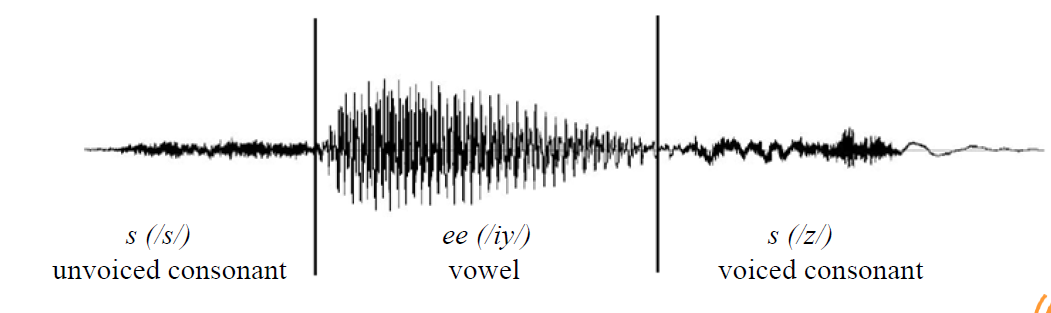
\includegraphics[scale=0.2]{Grafiken/bsp-sees.png}
	\end{itemize}
 		
\underline{Das Quelle-Filter-Modell} \\
	\begin{itemize}
		\item Wellengenerator: Periodische Schwingung der Stimmbänder
		\item Rauschgenerator: Luftstrom bei stimmlosen Phonen
		\item Systemmodell: Filtereigenschaft des Vokaltraktes (Mundraums)
		\item[] 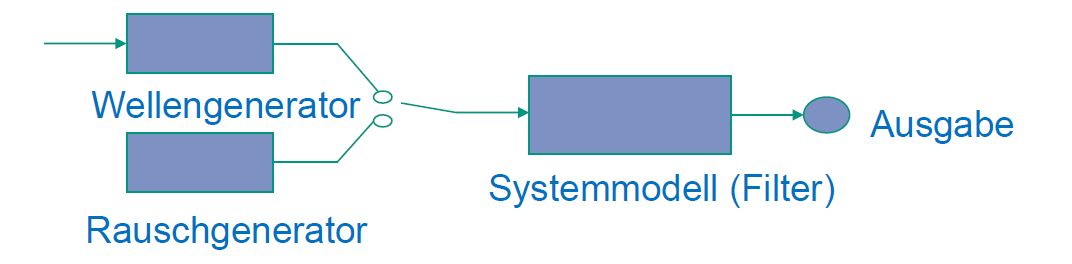
\includegraphics[scale=0.2]{Grafiken/quelle-filter-modell.png}
	\end{itemize}

\subsection{Akustische Phonetik und Phonologie}
\underline{Phonetik und Phonologie} \\
	\begin{itemize}
		\item Phonetik: Studium der Produktion, Klassifikation und Transkriptiopn von Sprachlauten -> Fokus liegt auf der akustischen Realisierung der Sprachlaute
		\item Phonologie: Studium der Verteilung und Struktur von Lauten in einer Sprache -> Hauptziel ist es, übergreifende Charakteristiken von Sprachlauten zu finden
	\end{itemize}

\underline{Phonetik} \\
	\begin{itemize}
		\item Artikulatorische Eigenschafen
			\begin{itemize}
				\item Laute können neben stimmhaft/stimmlos nach artikulatorischen Eigenschaften unterschieden werden
				\item Unterscheidung erfolgt entsprechend der Anatomie der wichtigen Artikulatoren und ihrer Position im Vokaltrakt
				\item Hauptkomponenten des menschl. Sprachproduk.apparats: Lungen, Trachea (Luftröhre), Pharynx (Rachen), Nasenhöhle und Mundhöhle. (Rachen + Mundhöhle = Vokaltrakt, Nasenhöhle = Nasaltrakt)
				\item Innerhalb des Vokaltrakts sind Stimmbänder, weicher Gaumen (Velum), harter Gaumen (Palatum), Zunge, Zähne und Lippen
			\end{itemize}
		\item Benennung von Sprachlauten
			\begin{itemize}
				\item Nasallaute:Luftstrom hauptsächlich durch Nase, gesenktes Velum (/n/)
				\item Orallaute: Luftstrom durch Mund, Velum verschließt Nasalraum
				\item Stoplaute (Plosive):Vokaltrakt kurzzeitig vollst. verschlossen (/p/, /b/)
				\item Frikative: Vokaltrakt teilw. verschlossen, Reibung entsteht (/f/)
				\item Approximanten: Vokaltrakt verengt, keine Reibung (/j/)
				\item Labial: Artikulationsort Lippen (/b/, /w/)
				\item Dental: Artikulation Zunge an Zähnen
				\item Alveolar: Alveole (Zahndamm) aktiv
				\item Palatal: Harter (vorderer) Gaumen aktiv
				\item Velar: Weicher (hinterer) Gaumen aktiv
				\item Glottal: Glottis, Stimmbänder aktiv (z.B. Be-amte)			
			\end{itemize}
		\item Konsonanten und Vokale
			\begin{itemize}
				\item Bei der Artikulation von Konsonanten befindet sich irgendwo im Vokaltrakt ein Hindernis (Stop, Verengung) für den Luftstrom
				\item Bei Vokalen liegt kein solches Hindernis vor
				\item Wichtige Eigenschaften für die Spracherkennung wichtig:
					\begin{itemize}
						\item Durschnittliche Dauer von Vokal ist viel länger als von Konsonant
						\item Vokale tragen den Hauptteil an Energie im Signal
						\item => Vokale wichtig für Spracherkennung, Konsonanten sind schwach und können mit Stille verwechselt werden
						\item Bei (englischem/deutschem) Text ist es gerade andersherum
					\end{itemize}
			\end{itemize}
		\item Modell des menschlichen Vokaltrakts
			\begin{itemize}
				\item Menschliche Vokaltrakt kann durch eine verlustfreie Röhre mit variablem Querschnitt approximiert werden
				\item Wichtige Approximation: Verkettung von endlichen vielen Röhren mit festen Querschnitt
				\item Mit dem Modell berechnen sich die Filereigenschaften des Vokaltrakts
				\item [] %G 12 - 18
			\end{itemize}
		\item Mathematische Beschreibung
			\begin{itemize}
				\item Unter geeigneten Bedingungen erfüllen Schallenwellen im Vokaltrakt die linearen partiellen DGLs
				\item "lossless tube"-Modell mit N Röhren approx. A
				\item analytische Lösung der DGLs möglich => Approximation der Frequenzantwort des Vokaltraktes
				\item Dieser Filter hat i.a. N konjugiert-komplexe Polstellen, die N/2 Resonanzfrequenzen (Formanten) entsprechen
				\item Tonhöhe der Formanten definieren den Laut
				\item Vokaltraktfilter kann durch ein nur-Pole-Modell, das nur Resonanzfrequenzen berücksichtigt, schon gut modelliert werden
			\end{itemize}
		\item Eigenschaften des Sprachspektrum
			\begin{itemize}
				\item Im Spektrum des Sprachsignals sind die Oberfrequenzen der Anregungsschwingung, die von den Stimmbändern kommt, besonders stark vertreten, so dass das Spektrum selber annährend periodisch ist
				\item Vokaltrakt wirkt als Filter auf die Anregung
			\end{itemize}
		\item Formanten
			\begin{itemize}
				\item Formanten lassen sich aus Spektrogrammen ablesen
				\item Die ersten beiden Formanten bestimmen im wesentlichen den Klang eines Vokals
			\end{itemize}
		\item Klassifikation von Vokalen: Formanten
			\begin{itemize}
				\item Das Vokaldreieck gibt an, welche Vokale im Mittel welche Formanten haben
				\item[] %G 12 - 23 rechts
			\end{itemize}
		\item Klassifikation von Vokalen: Formanten F1 und F2
			\begin{itemize}
				\item F1 entspricht der Hauptresonanzfrequenz des Rachenraumes
				\item F2 ist die Hauptresonanzfrequenz des Mundraumes
				\item Weg von Kehlkopf bis zur Zunge ist länger als Weg von Zunge bis Lippen => F1 < F2
				\item Zungenposition und Mundraum bestimmen die Werte F1 und F2
			\end{itemize}
		\item Diphtonge - Die charakteristischen Formanten F1 und F2 heißen auch formant targets, wenn
			\begin{itemize}
				\item Vokal ein spezifisches Ziel hat - Monophthong
				\item Zwei verschiedene Ziele kombinieren - Diphtonge
				\item Gibt einen fließenden Übergang zwischen den beiden Zielen
				\item Manche Sprachen (z.B. Mandarin) haben sogar Triphthonge 
				\item Diphtong wird i.d.R. genauso lang gesprochen wie ein Monophthong
			\end{itemize}
		\item Klassifikation von Konsonanten
			\begin{itemize}
				\item Werden durch Art und Ort der Artikulation beschrieben
				\item Artikulationsart - Mechanismus mit dem die Artikulation passiert
				\item Artikulationsort - Beschreibt Ort der Hauptverengung
				\item Sonorität (Schallfülle), Stimmhaftigkeit, Aspiration, Stärke
			\end{itemize}
		\item Vokaltraktformen: Plosive (Verschlusslaute)
			\begin{itemize}
				\item[] %G 12 - 28 + Spektogramm
				\item weiteres Plosiv: Glottal stop (Glottisschlag, Glottisverschlusslaut) - Luftstrom von den Stimmbändern im Kehlkopf gestoppt 
				\item Typisch: Kurzzeitig Luftstrom völlig unterbrochen
			\end{itemize}
		\item Vokaltraktformen: Nasale
			\begin{itemize}
				\item[] %G 12 - 13 +Spektogramm
				\item Mundraum komplett abgeschlossen und Rachenraum und Nasaltrakt miteinander verbunden
				\item Markante Eigenschaft: auffälligen fehlenden Frequenzbänder (gewisse Frequenzen im Mundraum werden vollständig reflektiert und so löschen sich Wellen aus)
			\end{itemize}
		\item Vokaltraktformen: Frikative (Reibelaute)
			\begin{itemize}
				\item[] %G 12 - 32 +Spektogramm
				\item Desweiteren gibt es glottalen Frikativ /h/ (wie in Haus) 
			\end{itemize}
		\item Phone und Phoneme
			\begin{itemize}
				\item Zwischen Schreibweise eines sprachl. Lautes und seiner Aussprache gibt es (prinzipiell) keinen Zusammenhang
				\item Phonetik: Sprachlaute haben keine inhärente Bedeutung
				\item Phonem: Kleinste Spracheinheit, die ein Wortpaar unterscheidet (minimales Paar) - Bsp: /kind/ != /rind/ -> /k/ und /r/ sind Phoneme
				\item Phon: Belieber Sprachlaut, der von anderen Sprachlauten akustisch unterschieden werden kann 
				\item Mit Phonem ist ein Bedeutungsunterschied verbunden und mit Phon nur ein akustischer Unterschied
				\item Schreibkonvention: /phonem/ vs [phon]
			\end{itemize}
		\item Phonetische Alphabete
			\begin{itemize}
				\item IPA: International Phonetic Alphabet (von der International Phonetic Association entwickelt + enthält Inventar für alle Laute aller Sprachen der Welt)
				\item Worldbet: 1-1 Abbildung von IPA-Symbolen auf ASCII-7 Symbole, um IPA-Alphabet auf Computern nutzbar zu machen
				\item Klein- und Großschreibung von Buchstaben hat auch Bedeutung
				\item Sampa: Basiert auch auf ASCII-7 Symbolen, wurde aber ursprünglich nur die deutsche und dann Indoeuropäische Sprachen entwickelt + Kürzlich auch auf weitere Sprachen ausgedehnt (X-Sampa)
			\end{itemize}
		\item IPA-Schema für Konsonanten + Vokale
			\begin{itemize}
				\item[] Konsonanten: %G 12 - 38
				\item[] Vokale: %G 12 - 39
			\end{itemize}
		\item Phone und Phoneme 
			\begin{itemize}
				\item Phoneme unterscheiden sich in Aussprachen durch:
					\begin{itemize}
						\item 1. Koartikulation, Kontext
						\item 2. Koartikulation bei variabler Sprechgeschwindigkeit
					\end{itemize}
				\item Wenn es mehrere Phone gibt, die dasselbe Phonem repräsentieren - heißt dann Allophone
			\end{itemize}
		\item Koartikulation
			\begin{itemize}
				\item Phoneme werden of auf systematische Weise von ihren Nachbarphonen beeinflusst
				\item Diesen Prozess bezeichnet man als Koartikulation
				\item In kontinuierlicher Sprache (mit variabler Sprechgeschwindigkeit)
					\begin{itemize}
						\item werden formant targets macnhmal nicht vollständig erreicht
						\item Betonungsmuster können verändert sein
						\item Laute können modifiziert werden (Assimilation)
						\item Laute können ganz verschwinden (Elision)
					\end{itemize}
				\item Effizientprinzip
					\begin{itemize}
						\item Sprecher versucht, den artikulatorischen Aufwand zu minimieren, ohne das dabei Information verlorengeht 
						\item Sprecher kann je nach Situation seinen Sprechgeschwindigkeit erhöhen 
					\end{itemize}
				\item Laute innerhalb einer Silbe beeinflussen sich mehr als benachbarte Laute in verschiedenen Silben
			\end{itemize}
		\item Prosodie 
			\begin{itemize}
				\item Eine Phrase kann, von der Intonation einzelner Laute abgesehen, auch als ganzes eine Melodie haben
				\item Eine Prosodie enthält Information über: Intention der Äußerung, Relevanz, Auflösung syntaktischen oder semantischen Zweideutigkeiten, Emotionen des Sprechers
				\item Prosodische Information ist: Intonation ("Melodie" des Satzes), Pausen, Betonung, Rhythmus
			\end{itemize}
	\end{itemize}

\subsection{Sprachperzeption}
\underline{Sprachproduktion und Sprachperzeption} \\
	\begin{itemize}
		\item Akustische Sprache pflanzt sich dann als Schalldruckwelle durch die Luft fort und wird vom menschlichen Ohr oder Mikrofon aufgefangen
	\end{itemize}
	
\underline{Sprachkommunikation von Mensch zu Mensch} \\
	\begin{itemize}
		\item[] %G 12 - 46
		\item A: Neurophysiologischer Prozess im Gehirn
		\item B: elek. Prozess in den efferenten Nervenbahnen
		\item C: Bewegung des Artikulationsapparates
		\item D: Erzeugung des akustischen Sprachsignals im Vokaltrakt
		\item E: Akustische Übertragung des Sprachsignals
		\item F: mechanischer Prozess im Mittelohr, hydromechanischer Prozess im Innenohr
		\item G: elek. Signale in den afferenten Nervenbahnen
		\item H: Neurophysiologischer Prozess im Gehirn des Empfängers
		\item I: Akustisches Feedback zum Ohr des Sprechers
	\end{itemize}
	
\underline{Physiologie des Ohres} \\
	\begin{itemize}
		\item Ohr empfängt die Schalldruckwellen aus der Luft
		\item Drucksignal wird in elek. Signal umgewandelt
		\item elek. Signal wird zum Gehirn weitergeleitet
		\item Außenohr:
			\begin{itemize}
				\item Ohrmuschen fängt durch ihre Form die Schallwelle ein und leitet sie in den Ohrkanal
				\item Orhkanal verstärkt das Signal
				\item Schließlich gelangt das Signal zum Mittelohr
				\item Signal Eingang + Ausgang: Schalldruckwelle in Luft
			\end{itemize}
		\item Mittelohr: 
			\begin{itemize}
				\item Schalldruckwellen bewegen das Trommelfell
				\item Dadurch gerät die Knochenstruktur (Hammer, Amboss, Steigbügel) in Schwingung 
				\item Durch das ovale Fenster wird eine Druckwelle der Flüssigkeit des Innenohres erzeugt
				\item Signal Eingang: Schalldruckwelle in Luft
				\item Signal Ausgang: Schalldruckwelle in Flüssigkeit
				\item Schalldruckwiderstand: Luft (niedrig), Flüssigkeit (hoch)
				\item Mittelohr übersetzt die Schallwelle von niedrigem Widerstand zu hohem Widerstand
				\item Knochenstruktur zwischen dem großen Trommelfell und dem kleinen ovalen Fenster dient als Verstärker
			\end{itemize}
		\item Innenohr:
			\begin{itemize}
				\item Die Cochlea ist eine spiralenförmige Röhre 
				\item Cochlea ist mit den Cochlea Filtern besetzt 
				\item Filter übersetzen die Wellen in Nervensignale
				\item Signal Eingang: Schalldruckwelle in Flüssigkeit
				\item Signal Ausgang: Elektrisches Signal im Gehörnerv
			\end{itemize}
		\item Cochlea:
			\begin{itemize}
				\item Cochlea Filter schwingen in den Wellen
				\item Filter sind mit der Basilarmembran verbunden
				\item Bewegung erzeugt eine Anregung in der Basilarmembran
				\item Dieses Signal wird dann durch den Gehörnerv an das Gehirn weitergeleitet
			\end{itemize}
	\end{itemize}

\underline{Wahrnehmung verschiedener Frequenzen} \\
	\begin{itemize}
		\item An verschiedenen Punkten entlang der Cochlea reagiert die Basilarmembran auf unterschiedliche Frequenzen
		\item Das Gehör basiert auf Frequenzen
	\end{itemize}

\underline{Physikalische vs. perzeptuelle Eigenschafen} \\
Gibt grundlegenden Unterschied zwischen der Wahrnehmung (Perzeption) eines Lautes und seinen messbaren physikalischen Eigenschaften. Manche physikalischen und perzeptuellen Eigenschaften hängen miteinander zusammen, sind aber keineswegs identisch
%G 12 - 55
	\begin{itemize}
		\item Unterschied: frequenzabhängige Wahrnehmung der Lautstärke (Empfindlichkeit variiert mit der Frequenz, Lautstärke != Intensität)
		\item Wahrnehmung hängt abvon: Resonanzfreq. des Gehörgangs, Übertragungsfunktion der Gehörknöchelchen
	\end{itemize}
	
\section{Sprackerkennung - Algorithmik}
\subsection{Sprachsignalverarbeitung}
Wir benötigen eine Repräsentation jedes Frames, die das enthaltene Sprachsegment möglichst gut charakterisiert
	\begin{itemize}
		\item Geringer Aufwand in Speicherplatz und Rechenzeit
		\item Verschiedene Phoneme sollen gut unterscheidbar sein
		\item Robust gegenüber Störungen 
	\end{itemize}

\underline{Speech Coding} \\
Wie repräsentiert man Sprache in digitaler Form?
	\begin{itemize}
		\item Direkte Speicherung der Wellenform (beachte Effekte von Sampling/Quantisierung, akustische Signal sollte zurückzugewinnen sein)
		\item Parametrische Repräsentation (gewisse Eigenschaften des Sprachsignals werden bezogen auf ein gewisses Modell gespeichert)
	\end{itemize}

Wie beurteilt man die Qualität einer Sprachcodierung?
	\begin{itemize}
		\item Qualität vs. Bitrate
		\item Benötigte Rechenleistung (Echtzeitanforderungen)
		\item Quantisierungsrauschen
		\item Robustheit bei weiteren Verarbeitungsschritten
		\item Fehlertoleranz
		\item Verhalten bei nichtsprachlichen Signalen
		\item Hohe Verständlichkeit für Menschen
	\end{itemize}
	
\underline{Sampling} \\
	\begin{itemize}
		\item Erster Schritt: A/D-Wandlung
		\item Hörbereich: ca. 200 Hz - 20 kHz
		\item Sprachsignal: ca. 300 Hz - 8 kHz
		\item Nach Nyquist-Theorem tasten wir in der Regel mit min. 16 kHz ab
		\item weniger problematisch ist die Quantisierung (16-bit-Quantisierung ist ausreichend für Spracherkennung)
	\end{itemize}
	
\underline{Mel-Frequency Cepstral Coefficients (MFCC)} \\
\underline{Framing (Fensterung} \\
Bei Framing gibt es 3 Dinge zu beachten:
	\begin{itemize}
		\item Frame Shift (die Schrittweite zwischen Frames)
		\item Frame Size (Fenstergröße)
		\item Fensterform
	\end{itemize}

Schrittweite ergibt sich aus Spracherzeugung und -perzeption:
	\begin{itemize}
		\item Sprechrate: 10-30 Phone/s => Phonem hat eine Länge von ca. 30 -100ms
		\item Jedes Phon kann aus mehreren Segmenten bestehen, üblicherweise wird es durch drei Zustände (Anfang, Mitte, Ende) modelliert
		\item Kleinstes Segment entspricht daher 10ms => Frame Shift ist deshalb 10ms
	\end{itemize}
	
\underline{Das Hamming-Fenster} \\
	\begin{itemize}
		\item Standardfenster in der Sprachsignalverarbeitung
		\item[] %G 13 - 12
		\item Fenstergröße beträgt etwa 1.5-2-fache des Frameshifts
		\item Typische Fenstergröße: ca. 16ms
	\end{itemize}
	
\underline{Fouriertransformation} \\
	\begin{itemize}
		\item Nächster Schritt zur Berechnung von MFCCs ist Frequenzanalyse der einzelnen Frames
		\item Zur Erinnerung: STFT
		\item[] %G Formel 12 - 15
		\item w[n] ist die Hamming-Fensterfunktion
		\item Die STFT erzeugt N Frequenzsamples aus N Zeitsamples - 1 komplexe Zahl pro Frequenz, Symmetrisch im Betrag + antisymmetrisch in der PHase => reicht die positiven Frequenzen zu betrachten
		\item Effiziente Berechnung: FFT (Fast Fourier Transform)
		\item Menschl. Ohr ist sehr empfindlich für die Phase des Audiosignals (aber nicht in 10-20ms Fenstern), daher reicht es in den Fenstern dieser Gröe das Amplitudenspektrum (Betrag des Spektrums) zu betrachten
	\end{itemize}
	
\underline{Mel-Filterbank} \\
	\begin{itemize}
		\item Betrachten wir uns die DTFT auf einem 16 kHz gesampelten Sprachframe, liefert -> 16ms entsprechen 256 Samples, gibt es 256 Frequenzkomponenten im Bereich von -8 kHz bis 8 kHz (aus Symmetriegründen sind 128 von ihnen interessant für uns)
		\item Problem: Diese Auflösung im Frequenzbereich ist viel zu hoch
		\item Es wäre besser, größere Frequenzbereiche zu betrachen
		\item Lösung: Vor der Logarithmierung verwenden wir eine Filterbank
		\item Filterbank fasst jeweils benachbarte Frequenzen gewichtet zusammen
		\item Filterbank orientiert sich am menschlichen Gehör (lin. Frequenzantwort zwischen 0 Hz und 1000 Hz, log. Antwort über 1000 Hz)
		\item Meistens benutzt: Mel-Filterbank (40 überlappende Dreiecksfilter zwischen 300 Hz und 8000 Hz + Verringert Dimensionalität des Signals auf 40 Koeffizienten pro Frame
	\end{itemize}
	
\underline{Cepstrum} \\
 	\begin{itemize}
 		\item Zunächst berechnen wir den Logarithmus des Amplitudenstpektrums (menschl. Gehör unterscheidet Frequenzen auch logarithmisch)
 		\item $e(t) * h(t) \rightarrow E(z) \cdot H(z) \rightarrow log E + log H$
 		\item Frequenzanalyse des logarithmierten Spektrums ergibt das Cepstrum
 		\item Einheit des Cepstrums ist die Quefrenz (auch Hz)
 		\item Cepstrum ist die Summe vom Einfluss der Anregungsschwingung und dem Einfluss vom Vokaltrakt (weil die FT linear ist)
 		\item Anregungsschwingung von 200 Hz im Beispiel sichtbar
 		\item[] %G 13 - 23
 	\end{itemize}
 	
\underline{Log-Mel-Spektrogramm} \\
	\begin{itemize}
		\item Mel-Filterbank behält die grobe Struktur des ursprünglichen Spektrogramm
		\item Durch anschließende Logarithmierung und inverser FT, erhält man die Mel-Frequency Cepstral Coefficients (MFCC)
		\item Überlicherwise werden die ersten 13-14 MFCCs verwendet
	\end{itemize}	
	
%G 13 - 25 		

\underline{Dynamik des Sprachsignals} \\
	\begin{itemize}
		\item Typischerweise werden etwa 14 Koeffizienten pro Frame extrahiert
		\item Nicht nur Betrag eines Koeffizienten ist interessant, sondern auch Änderungsrate (1. Ableitung) und "Beschleunigung" (2. Ableitung)
		\item Diese kann man wie folgt approximieren:
			\begin{itemize}
				\item Differenz zwischen Frames t und t-1 $\rightarrow$ "delta"-Koeffizienten, 1. Ableitung
				\item Differenz der deltas $\rightarrow$ "delta-delta"-Koeffizienten, 2. Ableitung 
				\item Alternativ kann man benachbarte Frames zeitverschoben "stacken"
			\end{itemize}
	\end{itemize}
	
\subsection{The Big Picture/Fundamentalformel der Spracherkennung}

\underline{Fundamentalformel der Spracherkennung} \\
	\begin{itemize}
		\item Gegeben eine Sequenz von Merkmalsvektoren X, finde wahrscheinlichste Wortsequenz W
		\item[] %G 13-32
	\end{itemize}
	
\underline{Automatic Speech Recognition} \\
	%G 13-34 
	\begin{itemize}
		\item Aussprache-Wörterbuch 
			\begin{itemize}
				\item Die Verbindung zwischen der Akustik und der geschriebenen Sprache (Beschreibe ein Wort als Konkatenation von Phonemen)
				\item[] %G 13-35
			\end{itemize}
		\item Akustisches Modell
			\begin{itemize}
				\item $p(X|W)$
				\item Gegeben W, mit welcher Warhscheinlichkeit wird die Merkmalssequenz X beobachtet?
			\end{itemize}
	\end{itemize}

\underline{Sprachproduktion als stochastischer Prozess} \\
	\begin{itemize}
		\item Das gleiche Wort/Phonem/Laut hört sich jedesmal anders an
			\begin{itemize}
				\item betrachte Wörter/Phoneme/Sprachteile als Zustände eines Sprachproduktionsprozesses
				\item diese Zustände haben unterschiedliche akustische Realisierungen
				\item wir können nur die Realisierung beobachten, nicht den Zustand
			\end{itemize}
		\item In einem Zustand können verschiedene Laute beobachtet werden, aber nicht alle Laute sind in jedem Zustand wahrscheinlich (in einem gegebenen Zustand emittiert der Sprachprozess einen Laut entsprechend einer bestimmten Wahrscheinlichkeitsverteilung/-dichte
		\item Produktionsprozess kann Übergänge aus einem Zustand in einen anderen machen, aber nicht alle Übergänge sind wahrscheinlich (Auch Zustandsübergänge folgen einer Wahrscheinlichkeitsverteilung)
	\end{itemize}
	
\underline{HMMs in der Spracherkennung} \\
	\begin{itemize}
		\item Ein typisches HMM (für das Wort "can")
		\item[] %G 13-39 
		\item 3-Zustands-Bakis-Modell pro Phonem
		\item Self-Loops erlauben beliebige Dauer eines Phonems
		\item Jeder Zustand modelliert Teil eines Phonems (Anfang, Mitte, Ende)
		\item Diesen Teil eines Phonems nennt man auch Subphonem
		\item Zustände, die zum selben "akustischen Phänomen" gehören, teilen sich ein Modell $Model S_1 = Model S_7 = Model g-b$ 
		\item[] %G 13-40
		\item Vorteile: Bessere Ausnutzung der Trainingsdaten, höhere Robustheit, bessere Parameterabschätzung, Rechenzeit wird gespart
	\end{itemize}

\underline{HMM-Training} \\
 	\begin{itemize}
 		\item 1. Init:	
 			\begin{itemize}
 				\item HMM muss initialisiert werden, vor dem eigentlich Training
 				\item Init alle Parameter zufällig oder identisch
 				\item Verwende gelabelte Daten (durch anderen Erkenner, manuell) - Init Gaussverteilungen z.B. mit K-Means o.ä.
 			\end{itemize}
		\item 2. Training / Iterative Optimierung 
			\begin{itemize}
				\item 1. Berechne Zustandsordnung (Forward-Backward, Viterbi)
				\item 2. Schätze HMM-Parameter neu (Baum-Welch, EM)
				\item Abbruchkriterien: keine Verbesserung der Scores (log-likelihoods) mehr auf Trainingsmenge oder separater Kreuzvalidierungsmenge, feste Anzahl Iterationen
			\end{itemize}
 	\end{itemize}
 	
\underline{Kontextabhängige Modellierung} \\
	\begin{itemize}
		\item Betrachte die Aussprachen von true, train, table und tell
		\item[] %G 13-42
		\item Die wahre Aussprache ist aber eher wie folgt
		\item[] %G 13-42
		\item Phonem T wird abhängig vom Kontext unterschiedlich ausgesprochen
		\item Erste Idee
			\begin{itemize}
				\item Eigentliche Aussprachen anstelle der Phoneme verwenden: /ch/ /r/ /uw/ statt /t/ /r/ /uw/
				\item Problem: /ch/ in true klingt anders als /ch/ in church
			\end{itemize}
		\item Zweite Idee
			\begin{itemize}
				\item Kontextabhängige Einheiten
				\item[] %G 13-43
			\end{itemize}
		\item[] $\rightarrow$ Trainiere unterschiedliche HMMs abhängig vom phonetischen Kontext
		\item Ein Phonem was von Vorgänger und Nachfolger abhängt ist ein Triphon
		\item Was passiert, wenn wir einheitlich jedes Phonem als Triphon modellieren? 
			\begin{itemize}
				\item Manche Kontexte kommen sehr selten vor (zu wenig Trainingsdaten!)
				\item Manche Kontexte kommen vielleicht im Trainingsmaterial gar nicht vor, aber könntne beim Decoding benötigt werden?
			\end{itemize}
		\item Ansatz: Fasse bestimmte Phoneme zu Klassen zusammen (Wissensbasiert: Artikulatorische Feature (Frikative, Vokale, etc. ))
		\item Triphone abhängig von diesen Klassen anstelle von einzelnen Phonemen
	\end{itemize}

\underline{CART} \\
	\begin{itemize}
		\item Verwende datengetriebene Methode, um Kontextklassen zu bilden
		\item CART steht für Classification und Regression Tree
		\item Aufteilung erfolgt durch binäre Fragen und deren Informationsgewinn
		\item Vorgehensweise
			\begin{itemize}
				\item Initial gibt es so viele Blätter im Baum wie Phoneme (Jedes Blatt enthält ein kontextunabhängiges Phonem)
				\item Iteratives vorgehen:
				\item 1. Bestimme Informationsgewinn jeder möglichen Frage für jedes Blatt im Baum
				\item 2. Spalte Blatt mit der Frage mit höchstem Informationsgewinn auf
			\end{itemize}
		\item Abbruchkriterien
			\begin{itemize}
				\item Maximale Anzahl Blätter
				\item Minimaler Informationsgewinn
				\item Minimale Menge an Trainingsdaten in jedem Blatt
			\end{itemize}
		\item[] %G  13-45
	\end{itemize}

\underline{Sprachmodellierung} \\
Was brauchen wir noch, um natürliche menschliche Sprache gut erkennen zu können?
	\begin{itemize}
		\item Lexikalisches Wissen: Vokabular, Aussprachewörterbuch
		\item Akustische Klassifikation haben wir gelernt: HMMs
		\item Wissen über die Sprache ist ebenso wichtig
			\begin{itemize}
				\item Ist eine Wortsequenz grammatikalisch korrekt (schwierig!)
				\item Hat eine Wortsequenz eine sinnvolle Bedeutung?
				\item Welche Worte sind jetzt wahrscheinlich?
				\item Wie kann man den Ablauf eines Dialogs verfolgen?
			\end{itemize}			 
	\end{itemize}
	
\underline{Stochastische Sprachmodelle} \\
	\begin{itemize}
		\item Modellieren Abfolge von Worten und Sätzen
		\item Gegebene Wortfolge W wird eine gewisse Auftrittswahrscheinlichkeit P(W) haben
		\item Sprachmodellierung ist in der Spracherkennung essentiell
			\begin{itemize}
				\item Weitere Informationsquelle beim Erkennungsprozess
				\item Hilft bei Unterscheidung von Homophonen
				\item Verringert den Suchraum 
				\item Erster Schritt zur semantischen Analyse
			\end{itemize}
		\item Schwierigkeit 1: Welche Wortsequenzen sind in gesprochener Sprache möglich?
			\begin{itemize}
				\item Klassische Methode zur Beschreibung: Formale Grammatik
				\item Aber wie beschreibt man die volle Flexibilität der deutschen Sprache?
			\end{itemize}
		\item[] $\rightarrow$ Wir brauchen eine probabilistische Methode, die ausdrucksstark, einfach aufzusetzen, und möglichst fehlertolerant ist
		\item Schwierigkeit 2: Anzahl möglicher Wortfolgen W wird sehr schnell sehr groß, wenn man die maximale Länge der Wortfolgen wachsen lässt
		\item $\rightarrow$ Brauchen eine effiziete Approximation von Sprachmodellwahrscheinlichkeiten (und einen guten Algorithmus)
	\end{itemize}
	
\underline{Wahrscheinlichkeit einer Wortsequenz} \\
	\begin{itemize}
		\item Wahrscheinlichkeit einer Wortsequenz P(W) kann zerlegt werden $P(W) = P(w_1 w_2 .. w_n) = P(w_1) \cdot P(w_2 | w_1) \cdot ... P(w_n | w_1 w_2 ... w_{n-1})$
		\item Wahrscheinlichkeit von $w_n$ hängt von allen Worten $w_1 w_2 ... w_{n-1}$ ab
		\item Vorberechnung aller Wahrscheinlichkeiten aller Wortfolgen unmöglich
		\item Mögliche Lösungen:
			\begin{itemize}
				\item $P(W|history)$ "on the fly" berechnen (selten, sehr teuer)
				\item Äquivalenzklassen von Historien bilden, um deren Anzahl zu reduzieren
			\end{itemize}
		\item Grammatik nur bei kleinen Vokabularen und beschränkter Domäne sinnvoll (z.B. Telefonservice)
	\end{itemize}

\underline{Sprachmodelle} \\
Verschiedene Methoden, Historien in Äquivalenzklassen einzuteilen
	\begin{itemize}
		\item Grammatische Eigenschaften
		\item POS (Part of Speech)
		\item Semantische Bedeutung der vorherigen Wörter
		\item Kontextgleichheit 
		\item Automatisches Clustering nach bestimmten Regeln
		\item Historie auf eine gewisse Anzahl Wörter beschränken (Unigramm, Bigramm, Trigramm)
	\end{itemize}

\underline{n-Gramm-Sprachmodelle} \\
Der übliche Ansatz, n-Gramm-Wahrscheinlichkeiten abzuschätzen:
	\begin{itemize}
		\item Suche Domänen spezifische Texte (Transkriptionen der Audiodaten des Trainings, Suche im Netz)
		\item bestimme Häufigkeit, mit der das Wort w nach einer Historie h auftritt
		\item zähle die Häufigkeit der Historie h im gesamten Text und normalisiere $P(w|h) = \frac{count(h,w)}{count(h)}$
	\end{itemize}
	
\underline{Automatic Speech Recognition - Suche} \\
	\begin{itemize}
		\item Suche: Akustik, Aussprachen und Sprache verbinden + gesprochene Sprache erkennen
		\item Um eine Sprachäußerung zu erkennen müssen alle möglichen Wortfolgen miteinander verglichen weren
		\item Die Gesamtheit aller möglichen Musterfolgen heißt Suchraum
		\item Typischer Suchraum hat extrem viele Elemente
		\item[] $\rightarrow$ Auswertung aller Wortsequenzen nicht möglich
		\item Benötigen Algorithmus der den Suchraum nur teilweise prüft und möglichst gute Hypothese findet 
		\item Dieses Problem nennt man Suche oder Decoding 
	\end{itemize}

\underline{Tiefensuche und Breitensuche} \\
	\begin{itemize}
		\item Tiefensuche
			\begin{itemize}
				\item Zu jedem Zeitpunkt wird nur der Pfad mit der höchsten Wahrscheinlichkeit weiterverfolgt (A* Suche) und Pfade werden zeitasynchron expandiert
				\item Vorteil: Suche findet für das gegebene Modell das optimale Ergebnis
				\item Nachteile: Unter Umständen müssen sehr viele Pfade expandiert werden + schlecht zu parallelisieren
			\end{itemize}
		\item Breitensuche (Standard-Suchmethode in der Spracherkennung)
			\begin{itemize}
				\item Expandiere die Pfade zeitsynchron und für jeden Frame werden nur eine feste/variable Anzahl an Pfaden weiterverfolgt (beam search)
				\item Vorteile: kann verschiedene Wissensquellen zeitsynchron kombinieren + gut parallelisierbar
				\item Nachteil: nicht garantiert, die optimale Lösung des Suchproblems zu finden
			\end{itemize}
	\end{itemize}
 

\section{Muskelaktivität - Einstehung, Messung (EMG), Anwendungen}
\subsection{Einstieg}

\begin{itemize}
	\item Ziel: Erfassung der menschlichen Bewegeung 
	\item Bewegungserfassung durch: visuelle Erfassung durch Kameras, direkte Erfassung der Bewegung, indirekt durch die Erfassung der Muskelaktivität die die Bewegung erzeugt
	\item Elektromyographie (EMG): Erfassung der elektrischen Potentiale, die durch Muskelaktivität entstehen
	\item Mensch-Maschinen-Schnittstelle: Erfassung von willentlichen Bewegungen
	\item Beschränkung auf die Betrachtung des Signals ab dem Rückenmark ($\alpha$-Motoneuronen)
\end{itemize}

\underline{Menschliche Bewegung} \\
Definition: Bewegungen sind räumliche Verschiebungen von Gewebe
	\begin{itemize}
		\item Größräumige Bewegungen z.b. Bewegungen der Beine beim Gehen
		\item Kleinste, fast unmerkliche Bewegungen z.B. Mimik
		\item Jegliche Bewegung geschieht durch Muskeln
			\begin{itemize}
				\item Quergestreifte Muskeln: Skelettmuskeln (Muskeln des Bewegungsapparates), Herzmuskel (unwillkürlich gesteuert)
				\item Glatte Muskeln: Muskeln der inneren Organe und Gefäße
				\item Augenmerk gilt den Skelettmuskeln
			\end{itemize}
	\end{itemize}

\subsection{Aufbau des Muskels}
	\begin{itemize}
		\item Bewegung und Muskelarbeit entsteht durch Muskelverkürzng (Muskelkontraktion)
		\item Elemente, die zur Kontraktion fähig sind, heißen Myofibrillen
		\item Skelettmuskeln sind über Sehnen mit dem Skelett (Knochen) verbunden
		\item Kleinste funktionelle Einheit des Skelettmuskels ist die Muskelzelle = Muskelfaserzelle = Muskelfaser 
		\item Muskelfasern schließen sich zu Faserbündeln zusammen, die man mit bloßem Auge als "Fleischfasern" erkennen kann
		\item Muskelfaser: 1/100 - 1/10 mm Durchmesser, Bis 20cm Länge
		\item Zytoplasma (Zellplasma) der Muskelfaser (Sarkoplasma) wird von der Membran (Sarkolmm) umschlossen
		\item Im Inneren der Muskelfaser befinden sich die Myofibrillen
		\item Nehmen größten Teil des Zellvolumens ein
		\item Myofibrillen: langestreckt, Durchmesser ca. 1 $\mu m$
		\item Myofibrillen sind in Zonen unterteilt
		\item Diese Zonen weiter unterteil in A-Bande (stark brechend) und I-Bande (schwach brechend)
		\item Innerhalb der I-Bande befindet sich die Z-Linie
		\item Bereich zwischen zwei Z-Linien: Sarkomer
		\item Unter dem Mirkoskop A/I-Bande als Querstreifen erkennbar - deshalb "quergestreifte Muskulatur"
		\item Myofibrillen bestehen aus 2 Typen von parallel gelagerten fadenartigen Filamenten: Myosinfilamente (langgestreckte Myosinmoleküle - Protein), Aktinfilamente (kugelförmiges Protein, kettenförmig gelagert verdrillt zu Faden)
		\item Beide Filamenttypen berühren sich, wo Ausstülpungen des Myosinmoleküls, die Myosinköpfe, das Aktinfilament berühren
		\item[] %G 14- 14 links unten
		
	\end{itemize}
%G Muskel aufbau

\subsection{Muskelkontraktion}
\begin{itemize}
	\item Folgender Vorgang läuft bei Muskelkontraktion ab:
		\begin{itemize}
			\item Aktivierung Myosin-Aktin-Querbrücke
			\item Verschiebung der Aktin- und Myosinfilamente in Längsrichtung gegeneinander (Filamentgleitmechanismus)
		\end{itemize}
	\item Sind minimale Verschiebungen, aber in vielen hintereinander Sarkomeren
	\item Insgesamt ergibt sich so eine beachtliche Längenverkürzung
	\item $\rightarrow$ Prozess nennt man Muskelkontraktion
\end{itemize}

Ausgangssituation:
	\begin{itemize}
		\item Muskeln in erschlafftem Zustand
		\item ATP (Adenosintriphosphat) gespalten in ADP + P und an Myosinkopf gebunden
		\item Bindungsstellen des Aktins mit Tropomyosin belegt
	\end{itemize}

Vorgang bei Erregung:
	\begin{itemize}
		\item Muskelfaser wird erregt, dadurch strömt $Ca^{2+}$ in die Muskelfibrillen
		\item Diese Depolarisierung breitet sich als Aktionspotential aus
		\item $Ca^{2+}$-Ionen binden sich an Troponinmoleküle $\rightarrow$ Tropomysin löst sich von Aktin-Bindungsstellen $\rightarrow$ Myosin kann an Aktin andocken
		\item ADP und P wurden freigesetzt $\rightarrow$ Myosinhals knickt um
		\item Myosinfilament zieht sich an Aktin entlang
		\item Muskel kontrahiert
	\end{itemize}

Nach der Kontraktion:
	\begin{itemize}
		\item ATP bindet sich an Myosinköpfchen
		\item ATP wird aufgespalten
		\item Durch Energie die bei der Spaltung in ADP + P frei wird, klappt Myosinkopf zurück in Ausgangsposition und löst sich von Bindungsstelle
	\end{itemize}
	
\underline{Neuromuskuläre Übertragung} \\
Woher kommt Erregung eines Muskels, die eine Kontraktion bewirkt?
	\begin{itemize}
		\item Aktivierung einer quergestreiften Muskelfaser erfolgt durch ein Motoneuron
		\item Spinale Motoneuronen = $\alpha$-Motoneuronen
		\item Axon des $\alpha$-Motoneuronen bildet Bündel mit anderen Axonen einen efferenten Nerv, der vom Rückenmark zur Peripherie läuft
		\item Axon endet in einer oder mehreren Synapsen, die an Muskel andocken - heißen motorische Endplatten
	\end{itemize}
	
\underline{Aktivierung einer Muskelfaser} \\
	\begin{itemize}
		\item Wenn das Motoneuron feuert, ensteht im Muskel ein Aktionspotential (MUAP)
		\item breitet sich längs der Muskelfaser vom Ursprung aus
		\item Führt zu Kalziumeinstrom
		\item Dieser führt zur Konformationsänderung der Myosinköpfe und somit zur Muskelkontraktion
		\item Zahl der von einem Motoneuron versorten Muskelfasern liegt zwischen 1 und mehreren Tausen
		\item Jede Muskelfaser hat nur eine Motorische Endplatte (d.h. wird von genau einem Motoneuron innerviert)
		\item Motorische Einheit (MU) = ein Motoneuron + alle von ihm innervierten Muskelfasern
		\item Um Muskelkontraktion aufrecht zu erhalten muss das Motoneuron wiederholt feuern, Abfolge von Aktionspotentialen (MUAPT)
		\item Intervalle zwischen den einzelnen MUAPs und MUAPT sind etwa gaussverteilt
	\end{itemize}
	
\underline{Kontraktionsstärke} \\
Die Stärke der Kontraktion hängt von Zahl der den Muskel versorgenden gleichzeitig feuernden Motoneuronen und von der Frequenz ihres Feuerns ab

\subsection{Elektromyographie (EMG)}
Elektromyograpie: Das Studium der Muskelfunktion durch Erforschung des elek. Signals, das die Muskeln erzeugen

\underline{Aktionspotentiale} \\
	\begin{itemize}
		\item Reizung der Muskelzelle erzeugt Aktionspotential in der Muskelfaser (MUAP)
		\item Aktionspotential entsteht durch Einstrom von Ionen in dne Muskel
		\item Durch das Aktionspotential entstehenden Potentialdifferenzen - invasiv und an der Hautoberfläche messbar
		\item Besonders an der Hautoberfläche: Überlagerung vieler Aktionspotentiale, Identifizierung einzelner Potentialquellen ist schwierige Aufgabe
		\item Betrachtung eines einzelnen Aktionspotentials an der Hautoberfläche: Plaziert man zwei Elektroden an zwei Positionen A (links) und B (rechts) auf dem Muskel (bipolare Ableitung)
			\begin{itemize}
				\item 1. Muskel in Ruhe: überall Ruhepotential, keine Differenz zwischen A und B
				\item 2. Muskel wird aktiviert, d.h. Aktionspotential AP entsteht
				\item 3. Da AP sich nur längs der Muskelfasern ausbreitet, wird die Elektrode nahe der Quelle A schneller von der Depolarisation erfasst als die quellferne Elektrode B $\rightarrow$ Potentialdifferenz A-B > 0
				\item 4. AP wandert weiter und erreicht nun Elektrode B $\rightarrow$ nun ist A-B < 0
				\item 5. AP wandert noch weiter, Potentialdifferenz ist wieder 0
			\end{itemize}
	\end{itemize}

\underline{EMG-Signal} \\
	\begin{itemize}
		\item Bei längerer Muskelkontraktion entsteht eine ganze Serie von Aktionspotentialen: MUAPT
		\item Unterschiede zwischen Signale durch Oberflächen- und Nadelelektrode: Oberflächen-EMG hat viel mehr Rauschen, Formen der einzelnen MUAPs eher schlecht erkennbar - erscheint tiefpassgefiltert
	\end{itemize}
	
\underline{Messung - Nadel- vs Oberflächenelektrode} \\
	\begin{itemize}
		\item Nadelelektrode: wird direkt in Muskel eingebracht
			\begin{itemize}
				\item Vorteile: spezifische + eng umrissene Aufzeichnungszone, erfasst auch kleine und tiefliegende Muskeln
				\item Nachteile: sind invasiv und erfordern sterile Bedingungen (nur durch Arzt einzubrinen), schwierig extakte Position wiederholt zu treffen
			\end{itemize}
		\item Oberflächenelektrode: 
			\begin{itemize}
				\item Vorteil: keine Schmerzen, Risiko
				\item Nachteil: Mehr Cross-Talk, schlechtere räumliche Auflösung
			\end{itemize}
		\item Nur Oberflächenelektroden im Bereich der Benutzerschnittstellen
	\end{itemize}
	
\underline{Muskel als Leiter} \\
	\begin{itemize}
		\item Relativ schlechter elek. Leiter
		\item Muskel wird als Tiefpassfilter
		\item Leitfähigkeit in Richtung der Muskelfasern höher als senkrecht zu ihnen
		\item Daten abgeleiterer Potentiale stark von der Elektrodenpositionierung abhängig
		\item Elektrodenabstand von der aktiven Faser spielt entscheidene Rolle
	\end{itemize}
	
\subsection{Anwedungsbeispiele}

\underline{Klinische Anwendung} \\
	\begin{itemize}
		\item Verhalten des Muskels bei gewissen wohldefinierten Reizen zu untersuchen
		\item exakt quantifizierbare Eigenschaften des Signals zu untersuchen
		\item nach Möglichkeit Verwendung von Nadelelektroden
		\item Erster Schritt von EMG in med./physio. Anwendungen ist oft Zerlegung des Signals in einzelne MUAPTs
		\item Algorithmus zur Zerlegung eines EMG-Signals:
			\begin{itemize}
				\item 1. Suche nach nächstem Peak im Rohsignal - dieser wird Knadidat für MUAP
				\item 2. Ordne diesen Peak einer Klasse von MUAPs zu bzw. erzeuge neue Klasse. Bei Bedarf kann ein menschlicher Experte eingreifen.
				\item 3. Nach erfolgreicher Zuordnung wird der Peak vom Rohsignal subtrahiert, Restsignal wird dann mit Schritt 1 weiterverarbeitet
			\end{itemize}
		\item Algorithmus bricht ab, wenn im Restsignal keine Peaks mehr vorhanden sind
		\item Algorithmus wird seit ca. 30 Jahren so verwendet
	\end{itemize}
	
\underline{Sonstige Anwedungen} \\
	\begin{itemize}
		\item Emotionserkennung
			\begin{itemize}
				\item Erkennung von Gesichtsausdrücken mittels EMG
				\item Warum? Nicht-invasive Methode, kleines Device, Elektroden einfach anzubringen
				\item Warum keine Videoerkennung? EMG in der Lage, Bewegungen aufzunehmen die auf Videos nicht sichbar sind + Mobiler kabelloser Rekorder kann überall mit hingenommen werden + benutzte Elektroden sind klein und leicht (nicht störend)
				\item Elektroden werden auf Muskeln plaziert, die an Gesichtsausdruck beteiligt sind
			\end{itemize}
		\item Erkennung von Fingerbewegungen
			\begin{itemize}
				\item Fingermuskulatur befindet sich am Unterarm
				\item Erlaubt Erfassung ohne Sensorik an der Hand
				\item Signale liefern auch Information über Kraft
				\item Problem: Crosstalk
			\end{itemize}
		\item EMG Prothesensteuerung/EMG-basierte Exoskelette
		\item FES- Funktionelle Elektrostimulation
			\begin{itemize}
				\item Verfahren zur Wiederherstellung der Bewegungsfunktion der Gliedmaßen
				\item Anwendungsgebiet: Lähmungen, bei denen nur Nervenbahnen zum betreffenden Muskel, aber nicht der Muskel selbst geschädigt ist
				\item Ziele: 1. Verhinderung von Muskelschwund und Sehnenkontraktion, 2. Steuerung des betreffenden Muskels
				\item Elektroden werden am Muskel angebracht (Oberflächenelektrode oder Implantat) $\rightarrow$ Übertragen elektrische Impulse an Muskel $\rightarrow$ Muskel kontrahiert
				\item Sensoren an gesunde Körperteilen anbringen 
				\item Erfassen der Bewegung $\rightarrow$ Übertragung auf defekten Muskel
			\end{itemize}
	\end{itemize}
 		
 		
 		
 		
 		
 		
 		
 		
 		
 		
 		
 		
 		
 		
 		
 		
 		
 		
 		
 		
 	

 
%%Ende
\end{document}